\UseRawInputEncoding
%% ReflectiveTun — Automation in Construction (cas-dc double-column template)

\documentclass[a4paper,fleqn]{cas-dc}

\usepackage[numbers]{natbib}
\usepackage{booktabs}
\usepackage{multirow}
\usepackage{array}
\usepackage{amsmath}
\usepackage{amssymb} % for \checkmark, \circlearrowright
\usepackage{algorithm}
\usepackage{algpseudocode}

\usepackage{graphicx}
\usepackage[dvipsnames]{xcolor}
\usepackage{hyperref}
\usepackage{placeins}
\usepackage{flafter} % prevent floats from appearing before their definition
\usepackage{float} % provides [H] to force a float to appear exactly here
\usepackage{caption}
\usepackage{subcaption} % provides subfigure environment
\usepackage{balance}
\usepackage{tikz}
\usetikzlibrary{arrows.meta,positioning,calc,fit}
% pgfplots optional; figures generated via scripts/drawing
% \usepackage{pgfplots}
% \pgfplotsset{compat=1.18}

% ─── Shared TikZ styles (reused across figures) ────────────────────────────
\tikzset{%
  box/.style={draw,rounded corners,align=center,minimum height=8mm,inner sep=4pt},
  gate/.style={draw,rounded corners,align=center,minimum height=10mm,inner sep=5pt},
  arrow/.style={-{Latex[length=2mm]}, thick}%
}

\usepackage{soul} % for \\hl
% Allow soul highlighting to contain common cross-reference commands
\soulregister\ref7
\soulregister\pageref7
\soulregister\eqref7
% Highlight helper that also works in math mode (e.g., $+36\%$)
\newcommand{\hlpct}[1]{\ifmmode\mbox{\hl{#1}}\else\hl{#1}\fi}
\usepackage[most]{tcolorbox} % for section-wide highlighting

% ─── Hidden subsection helper (keeps numbering/labels, hides printed title) ─
\makeatletter
\newcommand{\hiddensubsection}[1]{%
  \refstepcounter{subsection}%
  \addcontentsline{toc}{subsection}{\protect\numberline{\thesubsection}#1}%
  \@afterheading%
}
\makeatother

\providecommand{\printorcid}{}
\providecommand{\printfacebook}{}
\providecommand{\printtwitter}{}
\providecommand{\printlinkedin}{}
\providecommand{\printgplus}{}
\providecommand{\printinstagram}{}
\providecommand{\printemails}{}
\providecommand{\printurls}{}
\usepackage{lineno}
%\linenumbers % (disabled)

\begin{document}
\let\WriteBookmarks\relax
\def\floatpagepagefraction{1}
\def\textpagefraction{.001}

% ────────────────────────────── Front matter ──────────────────────────────

\shorttitle{Proxy4Tun: deployment-label-free proxy and reflective control for tunnel segmentation}
\shortauthors{X.\ Tao et~al.}

\title[mode=title]{Proxy4Tun: a proxy-guided reflective framework for deployment-label-free segmental tunnel lining segmentation}

\author[1]{Xinghui Tao}
\credit{Conceptualization, Methodology, Software, Writing -- original draft}

\author[1]{Guangming Wang}
\cormark[1]
\ead{gw462@cam.ac.uk}
\credit{Supervision, Writing -- review \& editing}

\author[1]{Brian Sheil}
\credit{Supervision, Funding acquisition, Project administration}

\cortext[cor1]{Corresponding author}

\affiliation[1]{organization={Construction Engineering, University of Cambridge},
    addressline={Trumpington Street},
    city={Cambridge},
    postcode={CB2 1PZ},
    country={United Kingdom}}

\begin{abstract}
Automated inspection of segmental tunnel linings requires accurate point-cloud segmentation, yet deployment rarely provides ground-truth (GT) labels for retuning or quality control. This paper presents \textbf{Proxy4Tun}, a framework that estimates segmentation quality without deployment labels. At design time, Bayesian-optimisation (BO) exploration of the bounded parameter space around one expert-tuned anchor per lining family generates 40 labelled trials per family (120 in total, all six pipeline stages tunable) spanning healthy to degraded configurations; feature ablation over GT-free evidence and coherence metrics distils this experience into a frozen five-feature Ridge proxy. At deployment, the proxy predicts mean Intersection-over-Union (mIoU) from intermediate pipeline artifacts alone, requiring only a family declaration and the segments-per-ring count. On 27 held-out Seg2Tunnel subsets (54 scored runs), the frozen proxy attains Spearman rank correlation 0.848 and mean absolute error 0.071, ranks the anchor above a known-bad configuration on 27/27 subsets, and flags all 27 known-bad runs with zero false alarms. A proof-of-concept self-refinement loop that selects LLM-proposed parameter overlays by proxy score improves mIoU on four of five subsets (gains $+$0.040 to $+$0.353). These results support calibrated intrinsic proxies as auditable, label-free control signals for tunnel-lining segmentation pipelines.
\end{abstract}

\begin{highlights}
\item Propose Proxy4Tun for label-free quality estimation of tunnel-lining segmentation.
\item Distil Bayesian-exploration trials into a frozen five-feature GT-free mIoU proxy.
\item Achieve Spearman 0.848 and MAE 0.071 on 27 held-out subsets.
\item Flag all 27 known-bad runs with zero false alarms.
\item Proxy-selected self-refinement improves mIoU on four of five subsets.
\end{highlights}

\begin{keywords}
Tunnel-lining segmentation \sep Point-cloud segmentation \sep Deployment quality control \sep Intrinsic proxy \sep Bayesian optimisation \sep Reflective LLM agents
\end{keywords}

\maketitle

\smallskip

\section{Introduction}\label{sec:intro}

Automated inspection of segmental tunnel linings supports structural health assessment under constrained access and high network scale~\cite{attard2018tunnelInspectionReview,montero2015roboticTunnelInspection}. Modern laser scanning yields dense measurements, but mixed structure, occlusions, and changing lining geometry make reliable segment-wise labelling difficult~\cite{huang2021bimMlUnderground,sjolander2023automatedTunnelInspections}. In practice, a deployed system must not only segment: without ground-truth (GT) labels it must also decide whether to \emph{accept}, \emph{refine}, or \emph{flag} each result.

\begin{figure*}[t]
\centering
\begin{subfigure}{0.98\textwidth}
{\raggedright\subsection*{Motivation}\vspace{-0.5\baselineskip}}
\centering

\includegraphics[width=0.8\textwidth]{figures/motivation.pdf}
\par\smallskip
(a)
\end{subfigure}

\vspace{4mm}

\begin{subfigure}{0.98\textwidth}
{\raggedright\subsection*{Position}\vspace{0.3\baselineskip}}
\centering

\includegraphics[width=1\textwidth]{figures/position.pdf}
\par\smallskip
(b)
\end{subfigure}

\caption{
Motivation and positioning of Proxy4Tun.
(a)~At deployment, tunnel segmentation outputs require accept, refine, or flag decisions without GT.
(b)~Existing approaches trade deployment adaptability against quality-control (QC) strength. Proxy4Tun targets strong QC with auditable adaptation by freezing a design-time intrinsic proxy and driving reflective refinement without deployment labels.
}
\label{fig:proxy4tun_motivation_positioning}
\end{figure*}

Existing tunnel point-cloud methods span auditable geometric pipelines~\cite{duan2021shieldTunnelLiningPointCloud,lin2024seg2tunnel}, supervised deep models that need large labelled corpora~\cite{qi2017pointnetpp,hu2020randlanet,wang2025tunnelnn}, and foundation-model pipelines such as SAM4Tun~\cite{ye2025sam4tun,kang2024samTunnelPointCloud,kirillov2023segmentAnything} that reduce annotation but remain sensitive to expert-tuned parameters. LLM-guided adapters (e.g.\ R4Tun) can retune parameters with structured context, yet they leave open the deployment-control question: \emph{how should the system know, without GT, that a candidate configuration is acceptable?} Medical and general vision quality-control literature provides reverse classification accuracy and related label-free checks~\cite{valindria2017rca,robinson2018segmentationQuality,fournel2021segmentationQC}, but these are not specialised to the failure modes of cylindrical tunnel unfolding---orientation collapse, hollow evidence, and circumferential phase errors---and do not expose an engineer-auditable accept/refine/flag decision tied to pipeline stages.

Proxy4Tun addresses this gap for a fixed unified SAM4Tun stage graph. Design-time BO exploration around one expert-tuned anchor per lining family is used only as an \emph{experience generator}: 40 space-filling trials per family (120 in total, with all six pipeline stages tunable) deliberately span healthy to degraded configurations so that GT-free intrinsic metrics can be related to mIoU across the whole quality range. Feature ablation over two metric groups---\emph{evidence} (artifact quality) and \emph{coherence} (result-form plausibility)---prunes ten candidates to a five-feature lean set, which is frozen into a single pooled Ridge proxy with a calibrated low-quality alarm. At deployment, scoring requires only intermediate pipeline artifacts plus a family declaration and the segments-per-ring count; no labels, per-tunnel tuning, or manual characterisation are used after calibration. A proof-of-concept (PoC) reflective loop then tests whether the proxy can select among LLM-proposed bounded parameter overlays.

This study contributes a quality-estimation mechanism, not a complete deployment system: absolute segmentation quality remains bounded by the underlying SAM4Tun stage algorithms and the single anchor per family, and the reflective loop is evaluated as a five-subset PoC. Within that scope, the evaluation isolates what a frozen linear proxy over stage-observable metrics can and cannot see.

This paper makes the following contributions:
\begin{enumerate}
\item A deployment-label-free quality-estimation formulation for segmental tunnel-lining segmentation that couples a GT-free intrinsic proxy over evidence and coherence features with accept/refine/flag decisions on a unified pipeline spanning staggered, continuous, and complex linings.
\item A design-time calibration protocol in which space-filling BO exploration around one anchor per family (40 trials each, all six stages tunable) is distilled by leave-one-out feature ablation and a permutation control into a frozen five-feature pooled Ridge proxy.
\item Holdout evidence on 27 unseen subsets (54 scored runs): Spearman 0.848 and MAE 0.071 against GT mIoU, 27/27 anchor-versus-bad ranking, and perfect known-bad flagging, with ablation evidence that feature pruning drives cross-family transfer and that pooling preserves alarm recall relative to per-family refits.
\item A PoC reflective loop in which LLM-proposed bounded overlays are selected by proxy score, improving mIoU on four of five subsets ($+$0.040 to $+$0.353); the single failure is traced to a stage-1 geometry defect invisible to the pruned feature set, delimiting the proxy's scope and motivating stage-1 auditing as future work.
\end{enumerate}

The rest of this paper is organised as follows. Section~\ref{sec:related} reviews related work on tunnel segmentation and deployment control. Section~\ref{sec:methods} presents methodology. Section~\ref{sec:results} reports results. Section~\ref{sec:discussion} discusses findings and limitations. Section~\ref{sec:conclusions} concludes.

\section{Related work}\label{sec:related}

This study situates Proxy4Tun among (i)~tunnel and infrastructure point-cloud segmentation, (ii)~deployment-time quality control without labels, (iii)~Bayesian optimisation as design-time experience generation, and (iv)~reflective LLM agents for iterative refinement. The distinguishing requirement is \emph{deployment control}: accept, refine, or flag a multi-stage tunnel pipeline when GT is unavailable.

\subsection{Tunnel and infrastructure point-cloud segmentation}

Tunnel inspection surveys motivate automated extraction of lining components from TLS and photogrammetry~\cite{attard2018tunnelInspectionReview,montero2015roboticTunnelInspection,sjolander2023automatedTunnelInspections}. Geometric and feature-engineered pipelines fit centrelines, unroll surfaces, and apply density or curvature rules~\cite{duan2021shieldTunnelLiningPointCloud,huang2021bimMlUnderground}; their logic is auditable but brittle when diameter, joint pattern, or density change. Supervised deep models on points---PointNet++~\cite{qi2017pointnetpp}, RandLA-Net~\cite{hu2020randlanet}, KPConv~\cite{thomas2019kpconv}, Mask3D~\cite{schult2023mask3d}---and tunnel-specific networks~\cite{ji2023spcnet,zhou2023aspcnet,zhang2022unrollingnet,wang2025tunnelnn} improve adaptability when labels exist, yet labelled tunnel corpora remain scarce and retraining is costly for each new lining family. Seg2Tunnel provides a public segmental-lining benchmark~\cite{lin2024seg2tunnel}. Foundation-model pipelines project tunnels to panoramic depth maps and prompt SAM~\cite{kirillov2023segmentAnything,kang2024samTunnelPointCloud}; SAM4Tun~\cite{ye2025sam4tun} achieves strong expert-tuned accuracy but exposes dozens of stage parameters that do not transfer off the reference. Proxy4Tun keeps that stage graph fixed and focuses on \emph{controlling} it at deployment rather than replacing the segmenter.

\subsection{Deployment-time quality control without labels}

When GT is absent, segmentation systems need secondary signals for reliability. Early work estimated segmentation error without labels~\cite{kohlberger2012segmentationError}; reverse classification accuracy and related QC scores similarly assess trustworthiness from model behaviour or image evidence~\cite{valindria2017rca,robinson2018segmentationQuality,fournel2021segmentationQC,cosarinsky2025inContextRCA}. Related work detects erroneous surface regions~\cite{zaman2023erroneousSurfaceRegions} or LiDAR perception failures~\cite{bogdoll2025lidarFailureDetection}, and uncertainty methods (dropout, ensembles, calibration) quantify predictive confidence~\cite{gal2016dropout,kendall2017uncertainties,lakshminarayanan2017deepEnsembles,guo2017calibration,vassilev2024uncertaintyInfrastructure}.
% TODO(refs): consider adding label-free model evaluation / accuracy prediction on unlabelled data
% (e.g. "predicting model performance under distribution shift", "AutoEval"), softmax-based failure
% prediction (Hendrycks & Gimpel style), and out-of-distribution detection surveys as further
% neighbours of this subsection once suitable bib entries are added.
These approaches rarely encode tunnel-specific failure modes---mirrored unrolls, fallback-heavy detections, or within-ring phase rotations---nor do they expose an engineer-auditable accept/refine/flag decision tied to pipeline stages. Proxy4Tun builds the control signal from \emph{intrinsic stage artifacts} of the tunnel pipeline itself, calibrated once against mIoU on a small design panel and frozen as a five-feature linear model whose coefficients an engineer can inspect.

\subsection{Bayesian optimisation for design-time experience}

Bayesian optimisation (BO) efficiently searches expensive black-box objectives with Gaussian-process surrogates and acquisition rules such as Expected Improvement~\cite{mockus1978bayesian,jones1998ego,rasmussen2006gpml,snoek2012practicalBO,shahriari2016reviewBO,frazier2018tutorialBO,garnett2023bayesianOptimization}. In Proxy4Tun, BO is \emph{not} the deployment optimiser, and the goal of exploration is not the optimum. The BO framework---bounded per-family search spaces around each anchor---is used as a design-time experience generator: scrambled-Sobol space-filling sampling of the search space populates a corpus of high-, medium-, and low-quality trials so that intrinsic features can be related to GT mIoU across the whole quality range, including deliberate failures. An acquisition-driven optimiser would concentrate samples near good configurations and starve the proxy of the degraded examples it must learn to flag.
% TODO(refs): consider adding quasi-Monte-Carlo / Sobol sequence references (e.g. Sobol 1967,
% Owen scrambling) and AutoML surrogate-benchmark literature once suitable bib entries are added.
The surrogate machinery is then discarded; only the frozen Ridge proxy and alarm threshold travel to deployment. This differs from using BO online on each new tunnel, which would reintroduce labels or an unverified surrogate at runtime.

\subsection{Reflective and agentic LLM refinement}

Reasoning-oriented LLMs support multi-step diagnosis via chain-of-thought and related protocols~\cite{wei2022chainOfThought,yao2023treeOfThoughts}. Self-Refine, Reflexion, and ReAct-style loops iterate on feedback without gradient updates~\cite{madaan2023selfrefine,shinn2023reflexion,yao2023react}, but they presuppose a feedback signal; in most engineering pipelines no such label-free critic exists.
% TODO(refs): consider adding LLM-agents-for-scientific/engineering-workflow references and
% reward-model / RL-from-proxy-feedback literature (the proxy as a learned reward) once suitable
% bib entries are added.
Proxy4Tun supplies that critic: in the PoC loop, an LLM agent prompted with the tunnel ontology inspects GT-free intrinsics and artifacts, proposes bounded multi-stage parameter overlays, and each round is scored by the frozen proxy, with the highest-scoring configuration retained. Unlike open-ended agent coding, the action space is the pipeline parameter schema; unlike one-shot LLM adapters, reflection is closed-loop on live artifacts. The same frozen proxy could in principle serve as a reward signal for reinforcement-learning-based tuning, which we leave to future work.

% ══════════════════════════════════════════════════════════════════════════
\section{Methodology}\label{sec:methods}
% ══════════════════════════════════════════════════════════════════════════

Our methodology defines the deployment-label-free quality-control task for segmental tunnel-lining segmentation, summarises the fixed unified SAM4Tun pipeline across lining families, and specifies the Proxy4Tun layer: design-time Bayesian optimisation (BO) that generates labelled experience, a ground-truth-free (GT-free) intrinsic proxy calibrated on that experience, and a staged reflective agent that reads the proxy together with an ontology-grounded context to propose bounded parameter updates. We then describe the feature-block ablation, Seg2Tunnel subset panel, holdout protocol, and metrics.

\subsection{Task definition}\label{sec:problem-def}

The upstream task is semantic segmentation of segmental tunnel linings from terrestrial laser scanning (TLS) point clouds. Given a raw point cloud of a tunnel section, each point is assigned a structural class label---background, key segment~(K), adjacent segments~(B), and standard segments~(A), with an additional class for seven-segment complex rings---following the Seg2Tunnel annotation schema~\cite{ye2025sam4tun}. The unit of analysis is a multi-ring subset.

A fixed expert configuration of the open-source SAM4Tun pipeline transfers poorly when lining layout, diameter, or scanning geometry depart from the tuning reference. At deployment, ground-truth (GT) labels are typically unavailable for either retuning or post-hoc quality control. Proxy4Tun addresses this gap: it does not alter the underlying stage algorithms, but learns a GT-free score that ranks candidate parameterisations and raises an alarm when a run is likely to be low quality. GT mIoU is used only at design time for proxy calibration and for offline evaluation of the proxy itself.

\subsection{Unified pipeline}\label{sec:pipeline}

\begin{figure*}[htp]
\centering
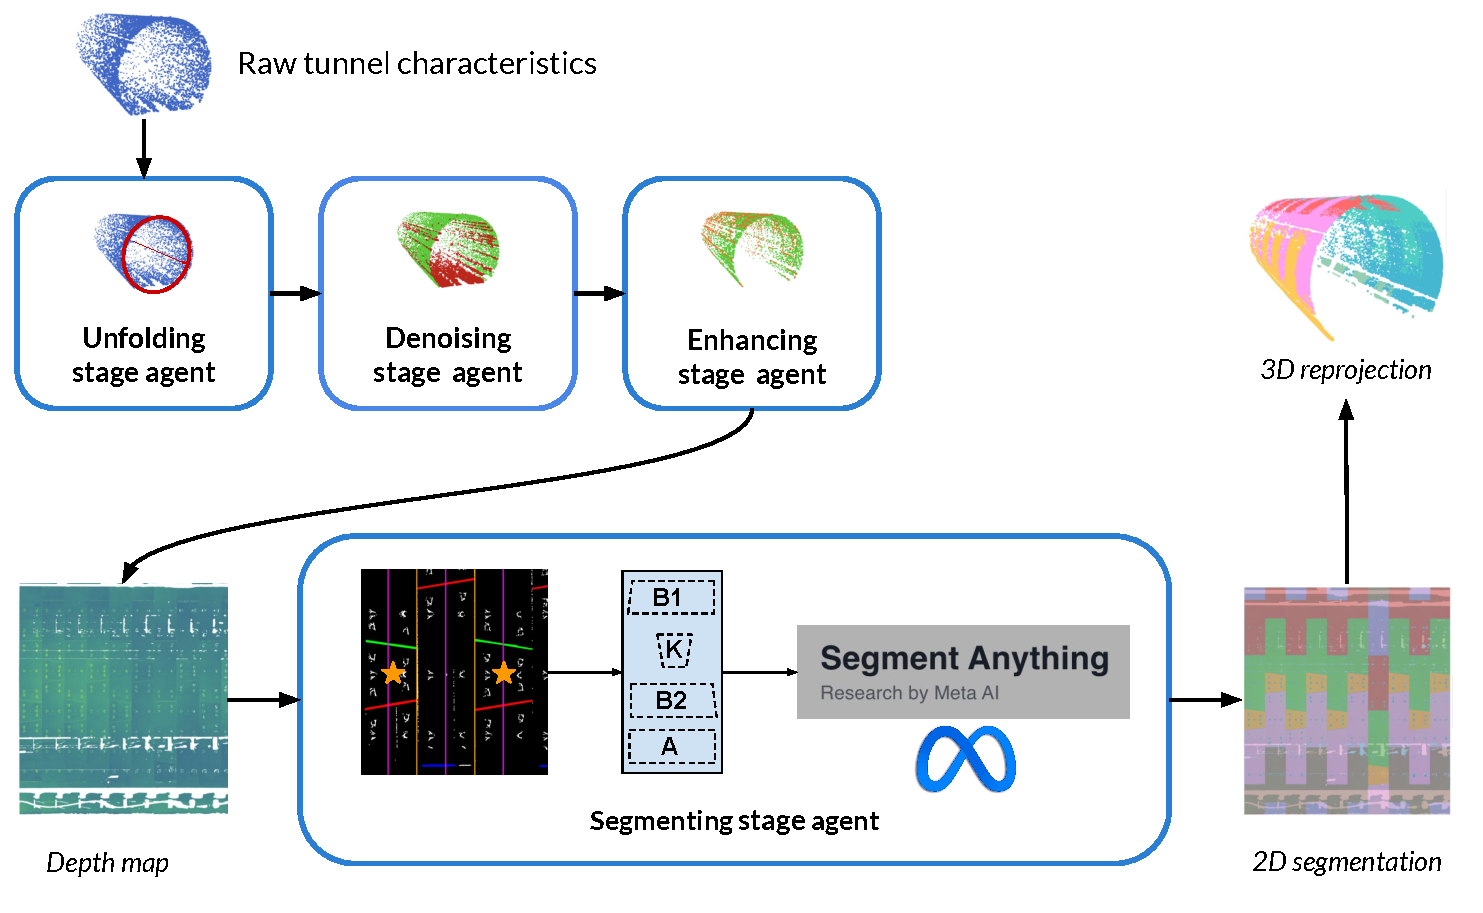
\includegraphics[width=0.95\textwidth]{figures/r4tun_pipeline.pdf}
\caption{Unified SAM4Tun stage chain used by Proxy4Tun. Stages~1--3 produce an oriented cylindrical frame and an enhanced panoramic depth map; Stage~4 detects joint lines and prompt centres; Stage~5 applies template prompts to SAM and reprojects masks to 3D. Family mode (\texttt{staggered}/\texttt{continuous}/\texttt{complex}) selects geometry priors and detection/SAM templates without changing the stage graph.}
\label{fig:unified-pipeline}
\end{figure*}

Proxy4Tun builds on a single unified stage graph (Fig.~\ref{fig:unified-pipeline}) that covers the three Seg2Tunnel lining families---staggered~(T1/T2), continuous~(T3), and complex interleaved~(T4/T5)---via a family-mode switch rather than separate code paths. Orientation knobs (e.g.\ circumferential handedness and ring-index sign) are frozen in the family parameter snapshots; BO and proxy evaluation then perturb only the tunable Stage~2--5 overlays. The stage algorithms remain fixed across all experimental conditions; only parameter values change.

\begin{figure*}[htp]
\centering

\includegraphics[width=0.8\textwidth]{figures/stage_u.pdf}
\caption{Stage~1---Unfolding. Left: fitted tunnel cross-section used to determine the reference centre and radius for cylindrical unfolding. Centre: 2D panoramic depth map derived from the 3D point cloud. Right: zoomed region of the unfolded map showing radial-distance encoding.}
\label{fig:stage-u}
\end{figure*}

\textbf{Stage~1---Unfolding} (Fig.~\ref{fig:stage-u}) establishes a cylindrical coordinate system. The point cloud is sliced at regular longitudinal intervals; each cross-section is fit by RANSAC ellipse estimation~\cite{fischler1981ransac}; ellipse centres are interpolated into a smooth centreline that defines the frame~$(r,\theta,h)$. The lining surface is projected into a panoramic depth map in which each pixel stores radial distance to the centreline. Residual recentring and sign conventions for~$h$ and~$\theta$ are treated as orientation invariants: a mirrored unroll can look geometrically clean while mapping every asymmetric class to its circumferential mirror, collapsing mIoU without an obvious cosmetic failure in the depth image.

\begin{figure*}[htp]
\centering

\includegraphics[width=0.8\textwidth]{figures/stage_d.pdf}
\caption{Stage~2---Denoising. Left: radial-distance distribution used to filter points outside the expected lining surface. Centre: unfolded depth map after filtering. Right: zoomed region of the denoised map.}
\label{fig:stage-d}
\end{figure*}

\textbf{Stage~2---Denoising} (Fig.~\ref{fig:stage-d}) removes non-structural artefacts by grid-based radial-density filtering inspired by DBSCAN~\cite{ester1996dbscan}, constrained by radial masks~$(R_\mathrm{low},R_\mathrm{high})$ (and, where applicable, angular masks). Dense connected regions are retained as lining; isolated points are rejected. The retained-point ratio and residual NaN structure of the depth map are primary evidence signals for the proxy.

\begin{figure*}[htp]
\centering

\includegraphics[width=0.8\textwidth]{figures/stage_e.pdf}
\caption{Stage~3---Enhancing. Left: curvature-guided surface and boundary interpolation with progressive upsampling. Centre: enhanced panoramic depth map. Right: zoomed views of the highlighted region.}
\label{fig:stage-e}
\end{figure*}

\textbf{Stage~3---Enhancing} (Fig.~\ref{fig:stage-e}) restores geometric continuity before detection. Local curvature guides point insertion: smooth panel regions are densified while high-curvature joints are preserved. Progressive upsampling and pixel-level outlier repair produce a depth map that balances panel continuity with sharp joint contrast---the input required by Hough detection.

\begin{figure*}[htp]
\centering

\includegraphics[width=0.8\textwidth]{figures/stage_p.pdf}
\caption{Stage~4--5---Detection and SAM segmentation. Hough-transform line detection~\cite{duda1972hough} recovers ring joints; template prompts for K/B/A (and the complex seventh class where applicable) are passed to SAM~\cite{kirillov2023segmentAnything}; 2D masks are reprojected to 3D via the stored pixel--point map.}
\label{fig:stage-p}
\end{figure*}

\textbf{Stages~4--5---Detection and segmentation} (Fig.~\ref{fig:stage-p}) recover joint lines with orientation-specific Hough thresholds, assemble prompt centres under the family layout grammar, and invoke SAM with template prompts. Masks are reprojected to per-point labels. Detection regularity (spacing, ring count, fallback rate) and SAM layout statistics (fill rate, completeness, segment-size variation, ontology divergence) form the coherence half of the proxy feature set.

The pipeline exposes dozens of tunable parameters across geometry, filtering, interpolation, detection thresholds, and SAM crop settings. In this study, family anchors provide warm-start configurations; exploration perturbs a bounded overlay spanning all six stages (family-specific search spaces, including stage-1 centreline knobs), while the orientation flags (circumferential handedness, ring-index sign) remain pinned to the canonical frame. A staged ontology of artifacts, quality metrics, failure modes, and remediation actions supplies the diagnostic vocabulary from which the intrinsic feature blocks below are distilled.

\subsection{Proxy4Tun}\label{sec:method}

\begin{figure*}[htp]
\centering
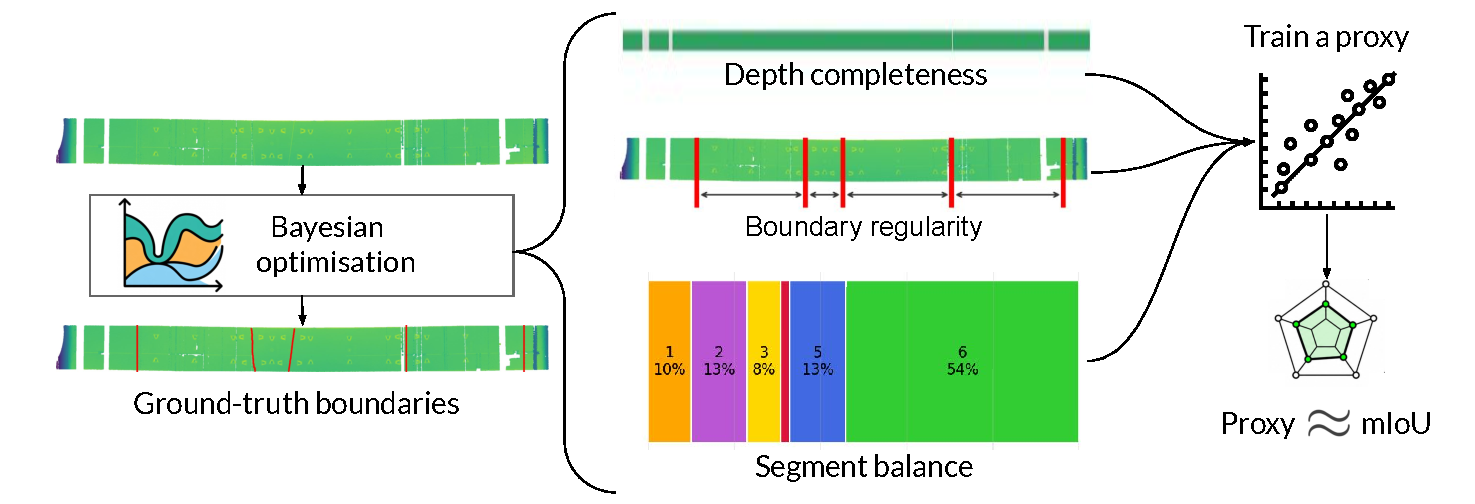
\includegraphics[width=0.95\textwidth]{figures/design-time.pdf}
\caption{Design-time Proxy4Tun workflow. Labelled family anchors generate Bayesian-exploration experience (parameters, GT-free intrinsic features, offline GT mIoU). Feature ablation and Ridge calibration freeze a single pooled deployment proxy and alarm threshold.}
\label{fig:design-time}
\end{figure*}

\begin{figure*}[htp]
\centering
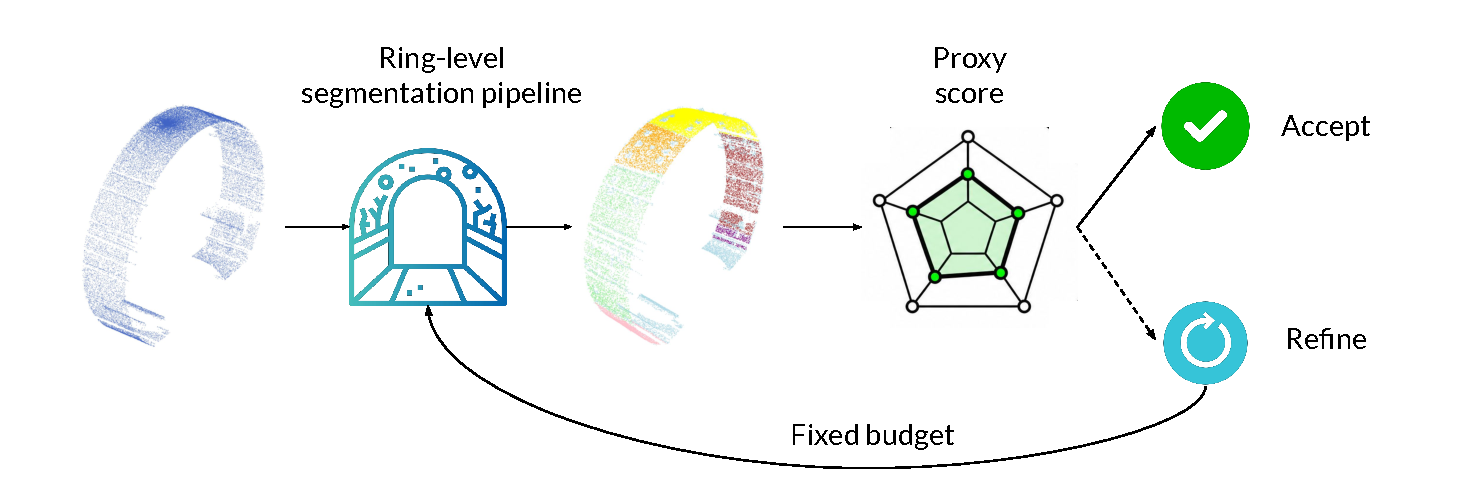
\includegraphics[width=0.95\textwidth]{figures/deploy-time.pdf}
\caption{Deployment-time Proxy4Tun workflow. A new subset is processed by the unified pipeline under a candidate parameter overlay. Intrinsic features feed the frozen proxy (score + alarm); a reflective agent may propose a bounded overlay and re-run within budget. No GT labels are required at deployment.}
\label{fig:deploy-time}
\end{figure*}

Proxy4Tun separates \emph{design time}, where a small labelled panel and BO trials are available, from \emph{deployment time}, where only pipeline artifacts may be observed (Figs.~\ref{fig:design-time}--\ref{fig:deploy-time}). The proxy provides a scalar GT-free score and alarm; the reflective agent (Section~\ref{sec:agent-design}) turns that signal, together with stage artifacts and ontology knowledge, into concrete parameter proposals.

\subsubsection{Intrinsic feature blocks}\label{sec:features}

Every completed run yields a vector of GT-free intrinsic metrics computed from stage artifacts. We organise the ten candidate metrics into two complementary groups aligned with the ontology's failure taxonomy (Table~\ref{tab:candidate-features}):

\begin{itemize}
\item \textbf{Evidence}---input and artifact quality across Stages~1--3: depth-map completeness (\texttt{depth\_nan\_ratio}), denoising retention (\texttt{denoise\_retained\_ratio}), and a stage-1 geometry audit pair (centreline recentring residual \texttt{unfold\_residual} and axis-orientation agreement \texttt{orient\_agreement}).
\item \textbf{Coherence}---structural plausibility of the detection and segmentation result (Stages~4--5): segment-mask fill rate, class-balance divergence from the equal-mass prior, the K-row detection residual and gate indicator, within-row anchor scatter, and cross-ring phase incoherence.
\end{itemize}

\begin{table*}[t]
\caption{The ten candidate features of the combined proxy P(e+c). Evidence
features audit input/artifact quality (Stages~1--3); coherence features audit
the structural plausibility of the detection and segmentation result
(Stages~4--5). All are computed from intermediate pipeline artifacts without
ground truth. The last column gives the standardised ridge weight for the five
features retained in the deployed lean model; pruned features are marked
``--''.}\label{tab:candidate-features}
\begin{tabular*}{\textwidth}{@{\extracolsep{\fill}} l l p{0.42\textwidth} c c @{}}
\toprule
Group & Feature & Meaning & Stage & Lean weight \\
\midrule
Evidence & \texttt{depth\_nan\_ratio} & Fraction of empty (white) pixels on the unfolded depth map. & 1--3 & $-$0.17 \\
Evidence & \texttt{denoise\_retained\_ratio} & Fraction of the point cloud surviving the radial denoising mask; high retention indicates under-filtering. & 2 & $-$0.39 \\
Evidence & \texttt{unfold\_residual} & Centreline recentring residual, $\log(1{+}\,\mathrm{cm})$ (stage-1 geometry audit). & 1 & -- \\
Evidence & \texttt{orient\_agreement} & Agreement $\lvert\mathrm{corr}(h, \text{PCA tunnel axis})\rvert$ between the unfolded axis and the point-cloud principal axis. & 1 & -- \\
\midrule
Coherence & \texttt{sam\_fill\_rate} & Fraction of points assigned a non-background segment label. & 5 & $+$0.47 \\
Coherence & \texttt{sam\_ontology\_divergence} & Total-variation distance between the predicted class-mass distribution and the equal-mass prior over segment classes. & 5 & -- \\
Coherence & \texttt{det\_row\_residual\_px} & Distance of detected K-row anchors from the design row pattern, $\log(1{+}\,\mathrm{px})$; meaningful only when gated. & 4 & $-$0.11 \\
Coherence & \texttt{det\_row\_gated} & Indicator that the K-row verification gate produced evidence for this run. & 4 & $+$0.13 \\
Coherence & \texttt{det\_row\_y\_std} & Within-row vertical scatter of K-row anchor points. & 4 & -- \\
Coherence & \texttt{phase\_incoherence\_deg} & Cross-ring circular distance of block-label ``clock faces''; detects per-ring label rotation. & 5 & -- \\
\bottomrule
\end{tabular*}
\end{table*}

Coherence features catch form and regularity failures; evidence features catch hollow or under-filtered runs that can still look locally regular. The deployed proxy does not use all ten candidates: leave-one-out feature ablation (Section~\ref{sec:comparators}) prunes the set to the five-feature \emph{lean} model whose standardised weights appear in Table~\ref{tab:candidate-features}. The phase-incoherence feature additionally powers an auxiliary alarm on regular linings (Section~\ref{sec:phase-alarm}).

\subsubsection{Bayesian-exploration experience generation}\label{sec:bo-experience}

Design-time exploration reuses the BO technical framework---bounded per-family search spaces $\Theta_f$ around each anchor configuration $P^{*}_f$---but its goal is \emph{coverage} of the quality range, not the optimum. Scrambled-Sobol quasi-random sampling of $\Theta_f$ generates candidate overlays spanning all six pipeline stages (including stage-1 centreline knobs); each candidate is materialised over the anchor parameters and run through the full pipeline, recording the GT mIoU $y_i$ and the intrinsic feature vector $\phi_i$ (Algorithm~\ref{alg:proxy_calibration}). Space-filling sampling is deliberate: an acquisition-driven optimiser would concentrate trials near good configurations and starve the proxy of the degraded examples it must learn to flag. Failed or feature-incomplete runs are excluded and topped up, yielding exactly $40$ valid trials per family ($120$ in total) that span healthy (mIoU~$\approx 0.87$) to collapsed (mIoU~$\approx 0.03$) configurations. Search-space bounds derive from the anchor values with modest padding, informed by parameter ranges observed during prior LLM adaptation and truncated where the pipeline fails structurally rather than gracefully. From each family we additionally freeze one \emph{known-bad} overlay (a historically low-mIoU trial far below the sibling-anchor floor) for holdout stress testing.

\subsubsection{Pooled lean Ridge proxy}\label{sec:ridge-proxy}

Let $\phi\in\mathbb{R}^{d}$ denote the intrinsic feature vector of a completed run and $y$ its GT mIoU. Features are standardised using the training mean $\boldsymbol{\mu}$ and scale $\boldsymbol{\sigma}$, and a single $\ell_2$-regularised linear regressor is fitted by cross-validated RidgeCV on the pooled $120$ trials from all three family anchors:
\begin{equation}
\hat{y}(\phi)
= \mathbf{w}^{\top}\!\left(\frac{\phi-\boldsymbol{\mu}}{\boldsymbol{\sigma}}\right) + b,
\label{eq:ridge-proxy}
\end{equation}
with regularisation strength selected on the training folds. Standardisation makes the coefficient magnitudes directly comparable, so the frozen weights (Table~\ref{tab:candidate-features}) double as a sensitivity record. The lean feature set is selected by leave-one-out ablation with leave-one-family-out cross-validation, and a permutation control (refitting on label-shuffled trials, $20$ repeats) verifies that the learned relationship exceeds Ridge capacity alone. Pooling is a deliberate design choice validated in the ablation: per-family refits of the same lean features are retained as a comparator (Section~\ref{sec:proxy-ablation-results}), but the pooled model triples the effective training data per family and preserves alarm recall.

An alarm threshold $\tau$ is calibrated on training predictions so that low proxy scores flag likely low-mIoU runs. At deployment, the frozen $(\hat{y},\tau)$ pair scores candidates without labels, requiring only the family declaration (which selects the class-count prior and gate applicability during feature extraction) and the segments-per-ring count. Figure~\ref{fig:proxy-training} shows the training fit; holdout fidelity is evaluated in Section~\ref{sec:main-results}. Algorithm~\ref{alg:proxy_calibration} summarises design-time calibration; Algorithm~\ref{alg:proxy_deploy} summarises deployment scoring.

\begin{figure}[t]
\centering

\includegraphics[width=0.62\columnwidth]{figures/proxy_training_fullstage.pdf}
\caption{Proxy training on the Bayesian-exploration corpus: proxy $\hat{y}$ versus GT mIoU on the $120$ trials ($40$ each from the staggered, continuous, and complex anchors; identity dashed). Train MAE~$=0.129$, Spearman~$\rho=0.853$.}
\label{fig:proxy-training}
\end{figure}

\begin{algorithm}[ht]
\caption{Design-time exploration and calibration of the GT-free proxy}\label{alg:proxy_calibration}
\begin{algorithmic}[1]
\Require Family anchors $\{P^{*}_f\}$; bounded search spaces $\{\Theta_f\}$ (all six stages); target count $N$; candidate features $F$ (Evidence $\cup$ Coherence)
\Ensure Frozen proxy $(\boldsymbol{\mu},\boldsymbol{\sigma},\mathbf{w},b,F_{\text{lean}})$ and alarm threshold $\tau$
\For{each family $f$} \Comment{Space-filling exploration (coverage, not optimum)}
    \State $U \gets \mathrm{SobolSequence}(|\Theta_f|, N)$; decode to bounded overlays $\{\theta_i\}$ on $P^{*}_f$
    \For{each candidate $\theta_i$}
        \State Run unified pipeline (Stages~1--5); record $\phi_i=F(\mathrm{artifacts})$, $y_i=\mathrm{mIoU}^{GT}$
    \EndFor
    \State $\mathcal{T}_f \gets$ trials with status ok and complete features; top up until $|\mathcal{T}_f|=N$
\EndFor
\State Pool $\mathcal{T} \gets \bigcup_f \mathcal{T}_f$; standardise features; fit RidgeCV on $\mathcal{T}$
\State $F_{\text{lean}} \gets$ leave-one-out ablation with leave-one-family-out CV \Comment{Smallest set preserving transfer}
\State Permutation control: refit on label-shuffled $\{y_i\}$; require real error $\ll$ permuted
\State Calibrate alarm threshold $\tau$ on training predictions; freeze all components
\State \Return $(\boldsymbol{\mu},\boldsymbol{\sigma},\mathbf{w},b,F_{\text{lean}},\tau)$
\end{algorithmic}
\end{algorithm}

\begin{algorithm}[ht]
\caption{Deployment-time proxy scoring}\label{alg:proxy_deploy}
\begin{algorithmic}[1]
\Require New subset; declared family $f$ and segments-per-ring count $C$; candidate overlays $\{\theta\}$; frozen proxy $(\hat{y},\tau)$; optional phase check
\Ensure Ranked scores; accept/alarm decision per candidate
\For{each candidate $\theta$}
    \State Run unified pipeline; compute $\phi=F_{\text{lean}}(\mathrm{artifacts})$ (no GT; $f$, $C$ set feature priors)
    \State $\hat{y}\gets\mathbf{w}^{\top}\big((\phi-\boldsymbol{\mu})/\boldsymbol{\sigma}\big)+b$; $\mathrm{alarm}_\mathrm{proxy}\gets[\hat{y}\le\tau]$
    \State $\mathrm{alarm}\gets\mathrm{alarm}_\mathrm{proxy}\lor\mathrm{alarm}_\mathrm{phase}$ \Comment{phase applicable on staggered/continuous only}
\EndFor
\State \Return scores/alarms; accept best safe candidate, else invoke Alg.~\ref{alg:reflective_adaptation}
\end{algorithmic}
\end{algorithm}

\subsubsection{Phase-coherence alarm}\label{sec:phase-alarm}

Intrinsic regression can miss a specific failure mode: within-ring \emph{block-label rotation}, where segment form is coherent and evidence ratios look healthy, yet the circumferential phase of labels is wrong relative to neighbouring rings. For staggered and continuous families we therefore add a GT-free phase check: each ring's predicted block clock is compared to its nearest peer rings; large clock-face disagreement raises $\mathrm{alarm}_\mathrm{phase}$. The deployment alarm is the logical OR of the proxy threshold and the phase check. Complex (T4/T5) rings lack a stable repeating phase prior under interleaved keys, so the phase check is marked inapplicable there.

\subsection{Reflective agent design}\label{sec:agent-design}

\begin{figure*}[t]
\centering
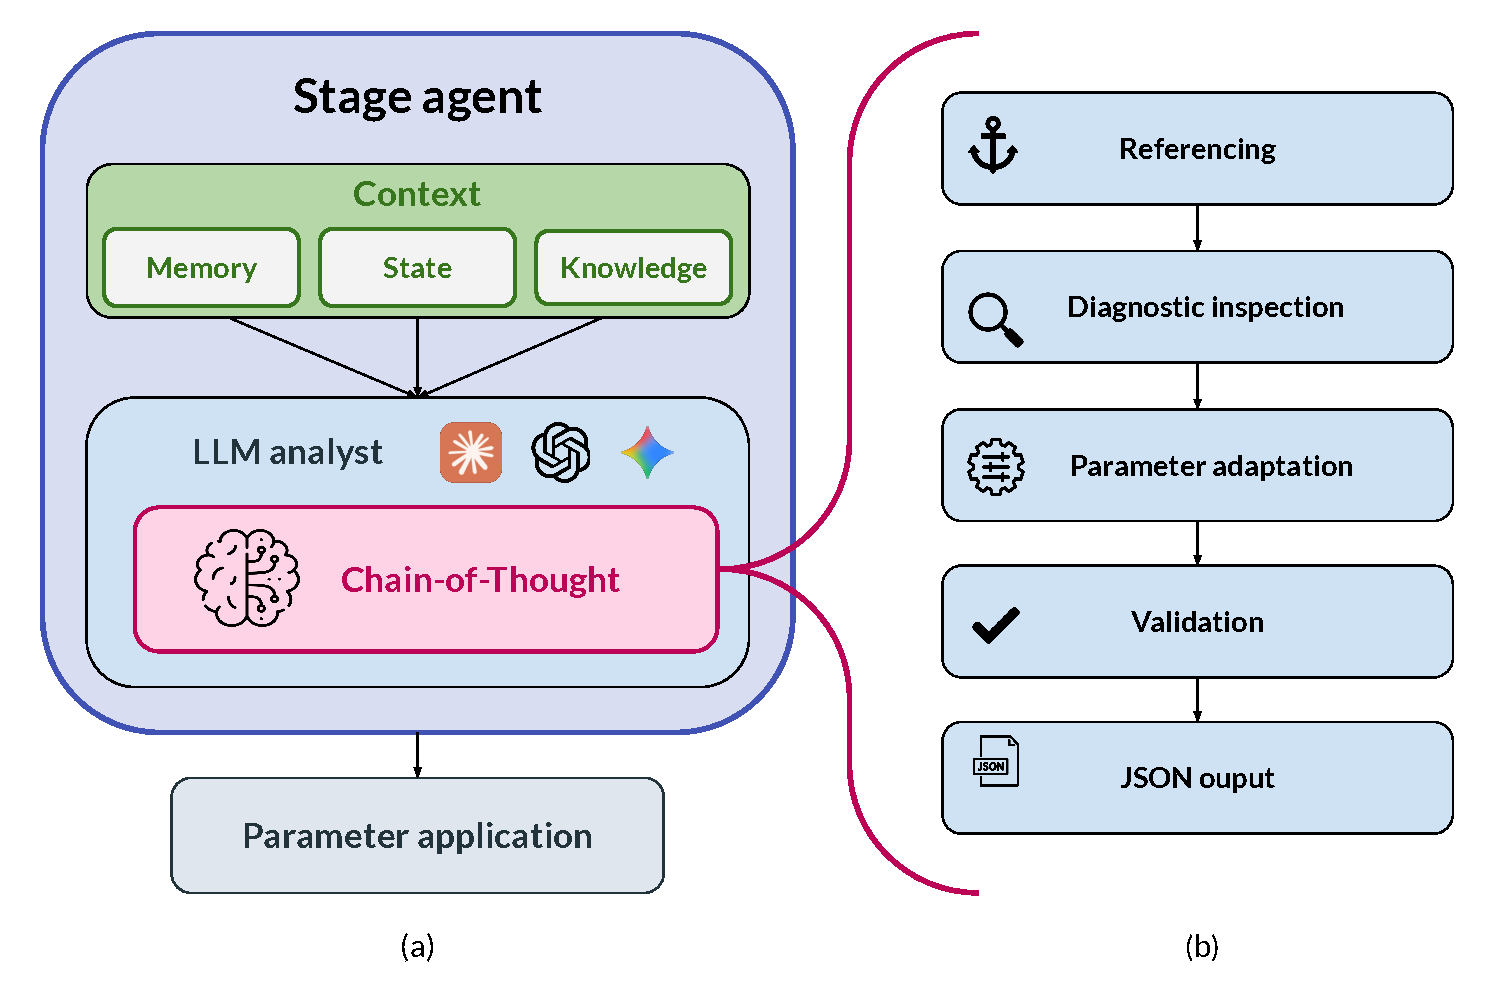
\includegraphics[width=0.8\textwidth]{figures/agent_design.pdf}
\caption{Reflective agent architecture in Proxy4Tun.
(a)~Each stage agent assembles a shared context (memory, state, knowledge, and the frozen proxy score/alarm) and an LLM analyst that performs structured reflection.
(b)~Reflection protocol: (1)~referencing family priors, (2)~diagnostic inspection against ontology rules and intrinsic metrics, (3)~upstream causal check, (4)~bounded parameter proposal, (5)~proxy-guided validation and JSON output.}
\label{fig:agent-design}
\end{figure*}

The proxy ranks and alarms; it does not by itself choose which parameters to change. Proxy4Tun therefore couples the frozen proxy to a \emph{reflective agent} layer that proposes bounded overlays without GT (Fig.~\ref{fig:agent-design}). One agent is associated with each pipeline stage. An analyst constructs the LLM prompt from the current context, invokes a fixed reflection protocol (Section~\ref{sec:reflection}), and parses a schema-conformant parameter JSON that the corresponding stage executes unchanged. After each round, intrinsic features and the proxy are recomputed; the agent may continue while budget remains and the proxy (and, where applicable, the phase alarm) indicate room for improvement. Stage scripts and evaluation code are identical across rounds---only the parameter overlay changes---and every proposal is logged with a textual rationale for engineer review or override.

Unlike R4Tun's one-shot per-stage adaptation from raw characteristics, reflection here is \emph{closed-loop}: each round observes live artifacts from the unified pipeline, scores them with the GT-free proxy, and may defer changes when an upstream failure is the likely cause. A reflection pilot freezes Stage~1 artifacts when comparing Stage~2--5 overlays so that centreline resampling does not confound attribution; unfolding overlays, when needed, trigger a full Stage~1--5 rerun.

\subsubsection{Context design}\label{sec:context-comp}

Each stage agent receives structured context with four components (Fig.~\ref{fig:agent-design}a).

\textbf{Memory} stores the family anchor: tunnel priors (diameter, radial/angular gates, segment grammar, key-layout mode) and the warm-start parameter snapshot for the sibling reference case. Memory is static within a reflection campaign and supplies the baseline against which live deviations are judged.

\textbf{State} is the cumulative post-stage summary for the current candidate: present artifacts, current parameter values, measured quality metrics (including the evidence/coherence intrinsic vector), the proxy score $\hat{y}$, proxy/phase alarms, and compact artifact descriptions (e.g.\ depth-map completeness, detected line count). State grows as stages execute and is prioritised over Memory when the two conflict, because it reflects geometry after upstream processing.

\textbf{Knowledge} comprises (i)~the staged ontology---artifacts, diagnostic rules, failure modes, remediation actions, and inter-stage dependencies---and (ii)~an experience document of empirically calibrated lessons (orientation invariants, anti-patterns such as chasing NaN fraction to zero, and the causal tuning order). Knowledge is authored once and shared across tunnels; numeric thresholds remain symbolic in the ontology and are interpreted relative to family-normal ranges in the experience notes.

\textbf{Proxy signal} injects the frozen Ridge score and alarms as first-class context. The agent is instructed to treat $\hat{y}$ as a \emph{directional} improvement signal: round-to-round $\Delta\hat{y}$ and corroborating artifacts take precedence over the raw score. A proxy increase driven only by evidence features while coherence degrades is treated as suspect (the pattern previously associated with cosmetic depth repairs that reduced GT mIoU).

\subsubsection{Reflection protocol}\label{sec:reflection}

Reflection follows a five-step protocol (Algorithm~\ref{alg:reflective_adaptation}; Fig.~\ref{fig:agent-design}b), with an explicit upstream-deferral step that R4Tun's one-shot CoT does not require:

\begin{enumerate}
    \item \emph{Referencing:} Compare the current tunnel's priors and warm-start parameters against Memory; note family mode (staggered / continuous / complex) and which Stage~1 orientation knobs are pinned.
    \item \emph{Diagnostic inspection:} Evaluate ontology diagnostic rules against State metrics and artifacts; emit matched failure modes. Prefer State over Memory on conflict. Check the phase alarm and permutation-shaped confusion signatures before attributing failure to detection or SAM.
    \item \emph{Upstream causal check:} Consult inter-stage dependencies. If a matched failure is likely caused upstream, defer to that stage's agent and do not retune local parameters in the current round.
    \item \emph{Bounded adaptation:} Propose an ordered list of remediation actions with concrete parameter deltas inside Knowledge bounds, respecting the causal priority used in experience: orientation $\rightarrow$ centreline/recentre $\rightarrow$ radial band $\rightarrow$ detection $\rightarrow$ SAM. Within a short reflection budget, early rounds confirm Stages~1--3 health before touching Hough or SAM geometry.
    \item \emph{Proxy-guided validation and JSON output:} Self-check logical constraints (e.g.\ $R_\mathrm{low}<R_\mathrm{high}$); reject proposals that flip pinned orientation knobs on a canonical frame; emit schema-conformant JSON. After execution, accept the round only if $\hat{y}$ improves (or alarm clears) without coherence collapse; otherwise revert and flag for review.
\end{enumerate}

\noindent\textbf{Notation for Algorithm~\ref{alg:reflective_adaptation}.}
$M$ is Memory (priors and warm-start $P_{\mathrm{ref}}$); $S$ is cumulative State; $K$ is Knowledge (ontology rules, bounds~$B$, dependencies~$D$, experience priors); $\hat{y}$ is the frozen pooled proxy; $R$ is the reflection budget in rounds.

\begin{algorithm}[ht]
\caption{Proxy-guided reflective parameter adaptation}\label{alg:reflective_adaptation}
\begin{algorithmic}[1]
\Require Subset; family $f$; Memory $M$; Knowledge $K$; frozen proxy $\hat{y},\tau$; budget $R$
\Ensure Accepted overlay $P^\star$ (or flagged baseline)
\State Run unified pipeline with warm-start; compute $\phi$, $\hat{y}\gets\hat{y}(\phi)$, alarms
\State $P^\star\gets P_{\mathrm{ref}}$; $\hat{y}^\star\gets\hat{y}$
\For{$r=1,\ldots,R$}
    \State \textbf{Phase 1--2:} Build State $S$; match diagnostic rules in $K$; list failure modes
    \State \textbf{Phase 3:} If any failure has likely upstream cause in $D$, set active stage $\leftarrow$ upstream; else local stage
    \State \textbf{Phase 4:} Propose $P_{\mathrm{proposed}}$ within bounds $B$ for the active stage (experience priority)
    \State \textbf{Phase 5:} Validate constraints; reject pinned-orientation flips; format JSON overlay
    \State Execute pipeline (freeze Stage~1 when overlay excludes unfolding); recompute $\phi',\hat{y}',\mathrm{alarms}'$
    \If{$\hat{y}'>\hat{y}^\star$ \textbf{and} coherence not degraded}
        \State $P^\star\gets P_{\mathrm{proposed}}$; $\hat{y}^\star\gets\hat{y}'$
    \Else
        \State Revert overlay; continue or stop if no safe improvement remains
    \EndIf
    \If{$\hat{y}^\star>\tau$ \textbf{and not} phase-alarmed}
        \State \textbf{break} \Comment{Accept}
    \EndIf
\EndFor
\State \Return $P^\star$ (flag for review if still alarmed)
\end{algorithmic}
\end{algorithm}

\subsection{Experimental setup}\label{sec:exp-setup}

\subsubsection{Dataset}\label{sec:dataset}

We use Seg2Tunnel multi-ring subsets spanning the three lining families (Table~\ref{tab:dataset}; Fig.~\ref{fig:tunnel_type}). Training experience comprises one labelled anchor case per family ($2$-$1$ staggered, $3$-$1$ continuous, $5$-$1$ complex), each explored with 40 space-filling trials over the bounded family search space (all six stages tunable), yielding $120$ trials in total. Holdout evaluation uses $27$ unseen subsets ($9$ per family, drawn from tunnels T1--T5), each scored under both the sibling-anchor configuration and the family's frozen known-bad overlay ($54$ scored runs). GT labels are used for offline mIoU and for proxy calibration only; they are never provided to the proxy at scoring time.

\begin{figure*}[t]
\centering
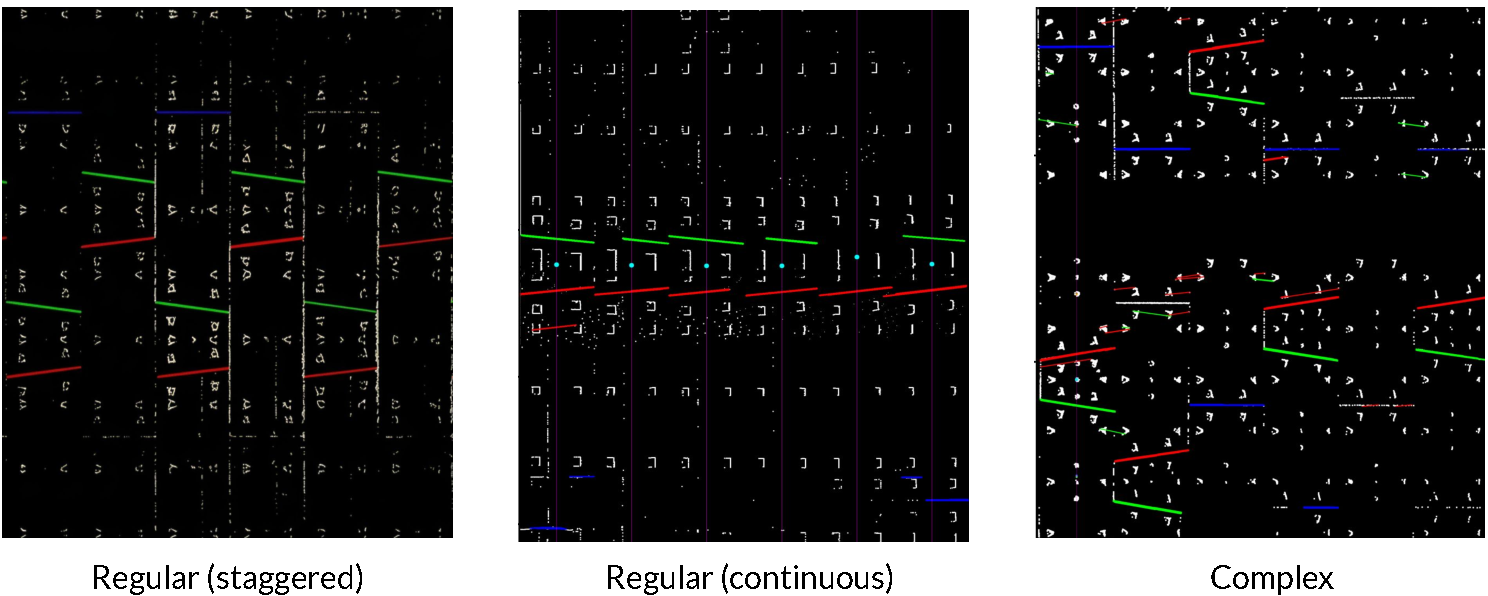
\includegraphics[width=0.8\textwidth]{figures/dataset.pdf}
\caption{Tunnel lining pattern categories. Left to right: staggered rings with a repeating key pattern; continuous rings with a fixed ring-wise order; complex rings with interleaved keys and no simple repeating phase.}
\label{fig:tunnel_type}
\end{figure*}

\begin{table*}[t]
\caption{Dataset and proxy-evaluation panel.}\label{tab:dataset}
\begin{tabular*}{\textwidth}{@{\extracolsep{\fill}} l l l l @{}}
\toprule
 & \multicolumn{2}{c}{Regular (T1, T2, T3)} & Complex (T4, T5) \\
\cmidrule(lr){2-3}\cmidrule(l){4-4}
Property & Staggered (T1, T2) & Continuous (T3) & \\
\midrule
Inner diameter & 5.5\,m & 5.9\,m & 7.5\,m \\
Ring length & 1.2\,m & 1.2\,m & 1.8\,m \\
Segments/ring & 6 & 6 & 7 \\
Joint type & Staggered & Continuous & Complex interleaved \\
Key-segment position & Ring-to-ring repeating pattern & Fixed ring-wise order & No repeating pattern \\
Scanning & Single-station & Multi-station & Single-station, offset \\
Eval.\ schema & 6-class & 6-class & 7-class \\
BO training anchor & $2$-$1$ & $3$-$1$ & $5$-$1$ \\
Holdout subsets & $1$-$1{\ldots}1$-$5$, $2$-$2{\ldots}2$-$5$ & $3$-$2{\ldots}3$-$10$ & $4$-$1{\ldots}4$-$5$, $5$-$2{\ldots}5$-$5$ \\
\bottomrule
\end{tabular*}
\end{table*}

\subsubsection{Experimental design}\label{sec:comparators}

The study follows a feature-set ablation that isolates each proxy component while holding the unified pipeline and holdout grid fixed (Table~\ref{tab:proxy-ablation}). All fits reuse the frozen $120$-trial training table and the $54$ holdout run manifests; no new pipeline runs are introduced during ablation. Conditions vary (i)~the feature set (evidence-only, coherence-only, combined, and the leave-one-out-pruned lean set) and (ii)~the model structure (one pooled Ridge on all $120$ trials vs.\ one Ridge per family on its $40$ trials, with identical lean features).

\begin{table}[ht]
\caption{Proxy ablation conditions.}\label{tab:proxy-ablation}
\begin{tabular*}{\tblwidth}{@{} c l >{\raggedright\arraybackslash}p{4.2cm} @{}}
\toprule
Level & Code & Condition \\
\midrule
1 & P(e) & Evidence only: 3D-to-2D projection quality \\
2 & P(c) & Coherence only: segmentation-structure consistency \\
3 & P(e+c) & Combined evidence + coherence \\
4 & Lean P(e+c) & Leave-one-out-pruned P(e+c), one model on all 120 trials \\
4a & \begin{tabular}[t]{@{}l@{}}Lean P(e+c) \\ per-family\end{tabular} & Same pruned features, one model per family (40 trials each) \\
\bottomrule
\end{tabular*}
\end{table}

As a capacity control, we permute mIoU labels within each family, refit the lean model, and repeat ($20$ shuffles). A large gap between real and permuted error indicates that the fit exploits genuine feature--mIoU structure rather than Ridge capacity alone. Train-parity and holdout gates on representative subsets verify that the unified pipeline reproduces the experience-generating anchors before proxy metrics are interpreted.

\subsubsection{Evaluation metrics}\label{sec:metrics}

Segmentation quality for offline analysis is measured by mean Intersection-over-Union (mIoU). For class~$c$,
\begin{equation}
\mathrm{IoU}_c = \frac{\mathrm{TP}_c}{\mathrm{TP}_c + \mathrm{FP}_c + \mathrm{FN}_c}, \qquad
\mathrm{mIoU} = \frac{1}{C}\sum_{c=1}^{C}\mathrm{IoU}_c,
\end{equation}
where $C=6$ for regular tunnels and $C=7$ for complex tunnels. Proxy quality is evaluated on the $27$ held-out subsets ($54$ scored runs) by:
\begin{enumerate}
\item \textbf{Absolute error}---MAE between $\hat{y}$ and GT mIoU, reported overall and stratified by family;
\item \textbf{Ranking accuracy}---whether $\hat{y}(\mathrm{anchor})>\hat{y}(\mathrm{bad})$ on each of the $27$ subset pairs;
\item \textbf{Alarm precision/recall}---treating known-bad runs as the positive alarm class;
\item \textbf{Spearman} rank correlation between $\hat{y}$ and GT mIoU on the holdout pool.
\end{enumerate}
The primary deployment criteria are perfect (or near-perfect) anchor-vs-bad ranking and high alarm precision: a false accept of a collapsed configuration is costlier than a modest calibration bias on already-acceptable anchors.

\section{Results}\label{sec:results}

We report (i)~overall proxy performance: calibration on the exploration trials and fidelity, ranking, and alarm behaviour on the held-out subsets; (ii)~feature-set and structure ablations with a permutation control; and (iii)~a proof-of-concept self-refinement loop driven by the frozen proxy. GT mIoU is used only offline.

\subsection{Overall performance}\label{sec:main-results}

\begin{figure*}[t]
\centering

\includegraphics[width=0.85\textwidth]{figures/proxy_holdout_fullstage.pdf}
\caption{Proxy prediction versus ground-truth mIoU on the 27 held-out subsets
(54 scored runs: sibling-anchor and known-bad configuration per subset). Each
point is one pipeline run scored by the frozen lean proxy; the dashed line
marks the alarm threshold $\tau = 0.495$. Runs below the threshold are flagged
as low quality. Colours indicate lining family.}
\label{fig:holdout-scatter}
\end{figure*}

Before assessing the proxy on held-out tunnels, we verified its calibration on
the 120 exploration trials. The frozen lean model reaches a training MAE of
0.129 and Spearman rank correlation $\rho = 0.853$ ($n = 120$;
Fig.~\ref{fig:proxy-training}). A permutation control confirms the learned
relationship is genuine: refitting on label-shuffled trials yields MAE
$0.271 \pm 0.009$ over 20 repeats, well outside the real model's error.
Leave-one-family-out cross-validation gives MAE 0.156 and $\rho = 0.717$,
indicating that the feature--quality relationship transfers across families
rather than memorising any single anchor.

\begin{table}[ht]
\caption{Proxy fidelity on the 27 held-out subsets (54 scored runs; frozen
lean model).}\label{tab:holdout-fidelity}
\begin{tabular*}{\tblwidth}{@{} l c c @{}}
\toprule
Metric & Full-stage & v2 reference \\
\midrule
Spearman $\rho$ & 0.848 & 0.810 \\
MAE (overall) & 0.071 & 0.071 \\
MAE (staggered) & 0.071 & 0.067 \\
MAE (continuous) & 0.064 & 0.066 \\
MAE (complex) & 0.076 & 0.080 \\
Bad-run flagging & 27/27 TP, 0/27 FP & 27/27 TP \\
\bottomrule
\end{tabular*}
\end{table}

\textbf{Predictiveness and calibration on held-out tunnels.}
Table~\ref{tab:holdout-fidelity} and Fig.~\ref{fig:holdout-scatter} summarise
deployment-time fidelity. Across the 27 held-out subsets (54 scored runs),
none of which contributed to calibration, the proxy ranks runs with
$\rho = 0.848$ and predicts absolute mIoU to within 0.071 on average.
Calibration is stable across families (MAE 0.064--0.076), supporting the
single-pooled-model design: one unified proxy serves staggered, continuous,
and complex tunnels with per-family errors within 0.012 of each other, so no
per-family recalibration is required at deployment.

\begin{figure*}[t]
\centering
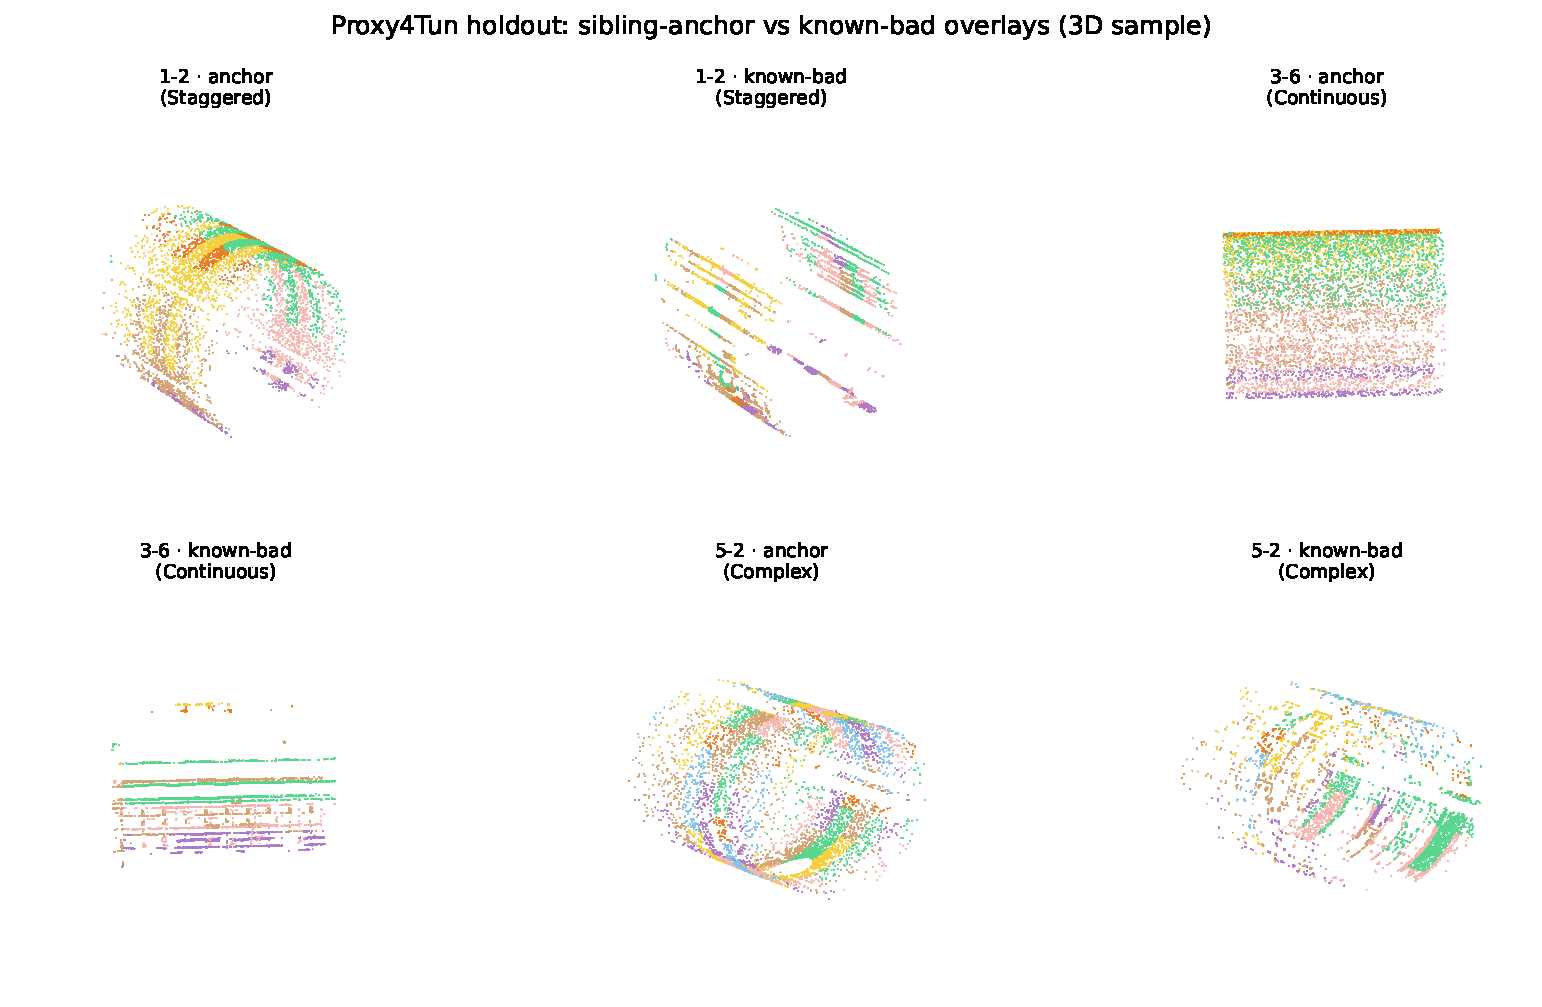
\includegraphics[width=0.98\textwidth]{figures/proxy4tun_3d_anchor_vs_bad.pdf}
\caption{Qualitative 3D samples on held-out subsets (staggered, continuous,
complex). Top: sibling-anchor configurations. Bottom: family known-bad
configurations. Points coloured by predicted segment class (background
suppressed). The proxy separates these regimes without access to labels.}
\label{fig:3d-anchor-bad}
\end{figure*}

\textbf{Blocking low-quality runs.} Used as an alarm at threshold
$\tau = 0.495$, the proxy flags all 27 known-bad runs while raising no false
alarms on the 27 sibling-anchor runs (Table~\ref{tab:holdout-fidelity});
anchor-versus-bad ranking is correct on all 27 subset pairs
(Fig.~\ref{fig:3d-anchor-bad} shows representative pairs). Given the size of
the flagged set we report raw counts rather than rates; the operating point
was fixed before holdout scoring and not tuned on the test subsets.

In practical terms, scoring a run is a five-feature linear evaluation over
artifacts the pipeline has already produced --- effectively free relative to
the pipeline run itself, and requiring no annotation. This is what makes the
proxy usable as an always-on acceptance gate and as a between-round selection
signal for iterative refinement (Section~\ref{sec:poc-verification}).


\subsection{Ablation analysis}\label{sec:proxy-ablation-results}

To isolate the contribution of each feature group, Table~\ref{tab:ablation-results}
and Fig.~\ref{fig:ablation-variants} report each ablation condition
(Table~\ref{tab:proxy-ablation}) under two regimes: training fit (Spearman
$\rho$ on the 120 calibration trials) and leave-one-family-out (LOLO)
cross-validation, in which the model is fitted on two anchors and evaluated on
the third. The LOLO columns are the ones that matter for deployment, since
they measure transfer to a family the model has not seen.

\begin{figure*}[t]
\centering
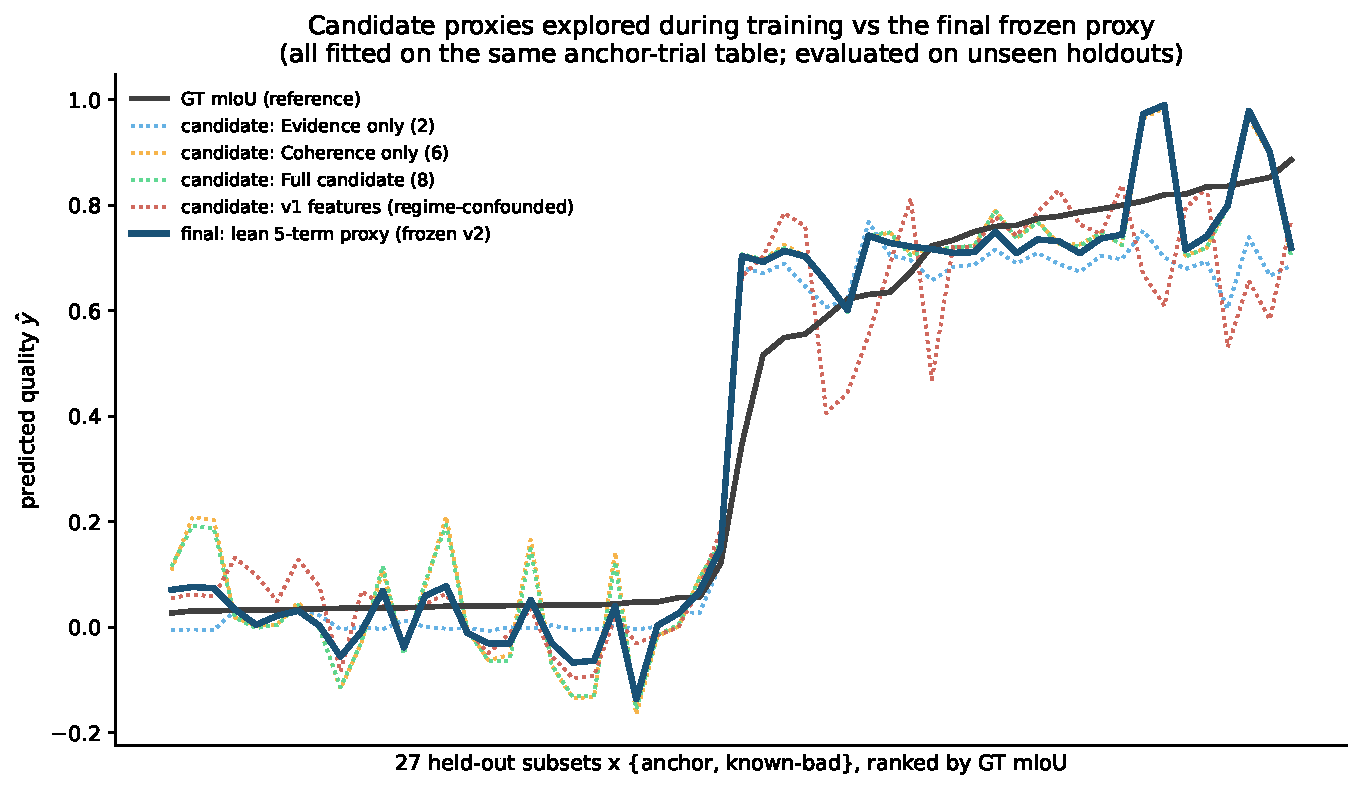
\includegraphics[width=0.85\textwidth]{figures/proxy_variants.pdf}
\caption{Feature-set ablation of the proxy. Bars compare evidence-only P(e),
coherence-only P(c), combined P(e+c), and the pruned lean P(e+c) under
training fit and leave-one-family-out cross-validation. Pruning, not
combination alone, delivers the best cross-family transfer.}
\label{fig:ablation-variants}
\end{figure*}

\begin{table*}[t]
\caption{Proxy feature-set ablation. Train $\rho$ is the Spearman correlation
on the 120 calibration trials; LOLO columns report leave-one-family-out
cross-validation.}\label{tab:ablation-results}
\begin{tabular*}{\textwidth}{@{\extracolsep{\fill}} l c c c c @{}}
\toprule
Condition & \#Features & Train $\rho$ & LOLO $\rho$ & LOLO MAE \\
\midrule
P(e) (evidence only) & 4 & 0.682 & 0.429 & 0.405 \\
P(c) (coherence only) & 6 & 0.837 & 0.643 & 0.160 \\
P(e+c) (combined) & 10 & 0.876 & 0.537 & 0.346 \\
\quad $-$ \texttt{sam\_fill\_rate} & 9 & 0.700 & 0.198 & 0.415 \\
Stage-1 features only & 2 & 0.212 & $-$0.007 & 0.325 \\
\textbf{Lean P(e+c) (deployed)} & \textbf{5} & \textbf{0.853} & \textbf{0.717} & \textbf{0.156} \\
\bottomrule
\end{tabular*}
\end{table*}

\textbf{Evidence alone is insufficient.} The evidence-only proxy P(e) tracks
artifact quality (depth-map completeness, denoising retention, stage-1
geometry) but correlates only weakly with final segmentation quality
($\rho = 0.682$ train, 0.429 LOLO). Artifact quality is a necessary but not
sufficient condition: a run can produce a clean depth map and still assign
segment labels with the wrong structure.

\textbf{Coherence carries most of the signal.} The coherence-only proxy P(c)
reaches $\rho = 0.837$ on training trials and generalises markedly better than
evidence alone (LOLO MAE 0.160 vs.\ 0.405). Features describing the
\emph{form} of the result --- segment fill rate, class balance, and K-row
detection consistency --- are the primary carriers of quality information,
led by \texttt{sam\_fill\_rate}: removing this single feature from the
combined set collapses cross-family transfer ($\rho_{\text{LOLO}}$ 0.537
$\rightarrow$ 0.198).

\textbf{Combination helps in-sample; pruning is what makes it transfer.} The
full combined set P(e+c) achieves the best training fit ($\rho = 0.876$) but
generalises \emph{worse} than coherence alone (LOLO $\rho = 0.537$),
indicating that the weaker features overfit anchor-specific regularities.
Leave-one-out pruning to the five-feature lean set restores and surpasses
both: LOLO $\rho = 0.717$ and MAE 0.156, the best transfer of any condition.
The lean model is therefore not merely a parsimony choice --- pruning is
itself the mechanism that converts in-sample fit into cross-family
generalisation. On standardised inputs its coefficients are directly
comparable: \texttt{sam\_fill\_rate} dominates ($+0.47$), followed by
\texttt{denoise\_retained\_ratio} ($-0.39$), \texttt{depth\_nan\_ratio}
($-0.17$), and the K-row pair (\texttt{det\_row\_gated} $+0.13$,
\texttt{det\_row\_residual\_px} $-0.11$). The negative weight on
\texttt{denoise\_retained\_ratio} is physically expected: effective denoising
must remove non-lining clutter, so a high retention ratio marks under-filtering
(clutter surviving the radial gates) and correctly predicts lower mIoU.

\textbf{Stage-1 features do not survive pruning.} Included as evidence
candidates for the first time in this campaign, the two stage-1 audit features
(centreline residual, orientation agreement) carry almost no standalone signal
($\rho = 0.212$ train, LOLO $\approx 0$) and are pruned from the lean set.
This is an honest boundary of the current proxy: stage-1 geometry defects are
not visible to it, which is precisely the failure mode isolated by the 4-3
case study (Section~\ref{sec:main-results}) and the motivation for stage-1
gating in future reflective agents.

\begin{table*}[t]
\caption{Unified versus per-family lean P(e+c) on the 120-trial full-stage
table (same five features; 40 trials per family). Holdout: 27 subsets, 54
scored runs.}\label{tab:unified-vs-perfamily}
\begin{tabular*}{\textwidth}{@{\extracolsep{\fill}} l c c c c @{}}
\toprule
Model & MAE & Spearman $\rho$ & Rank & Alarm P/R \\
\midrule
Lean unified (pooled) & 0.071 & 0.848 & 27/27 & 1.00 / 1.00 \\
Lean per-family & 0.057 & 0.872 & 27/27 & 1.00 / 0.96 \\
\bottomrule
\end{tabular*}
\end{table*}

\textbf{Unified versus per-family.} Refitting the same lean features as three
family-specific Ridge models (40 trials each) versus one pooled model
(120 trials) yields Table~\ref{tab:unified-vs-perfamily}. Per-family
calibration edges the pooled model on absolute fidelity (MAE 0.057 vs.\ 0.071;
$\rho$ 0.872 vs.\ 0.848), while both achieve perfect anchor-versus-bad ranking
(27/27). The pooled model retains perfect alarm recall (1.00 vs.\ 0.96; one
missed low-mIoU run under per-family thresholds). We therefore deploy the
unified model: the fidelity gap is small ($+$0.014 MAE), a single calibration
is operationally simpler, and alarm recall is undiminished. Earlier unbalanced
per-family fits (14/35/14 rows) had already shown that starving family-specific
models harms alarm recall more than it helps MAE; the balanced 40/family design
closes the MAE gap but does not overturn the case for pooling.


\subsection{Proof-of-concept verification: the proxy as a self-refinement signal}\label{sec:poc-verification}

\begin{figure*}[t]
\centering
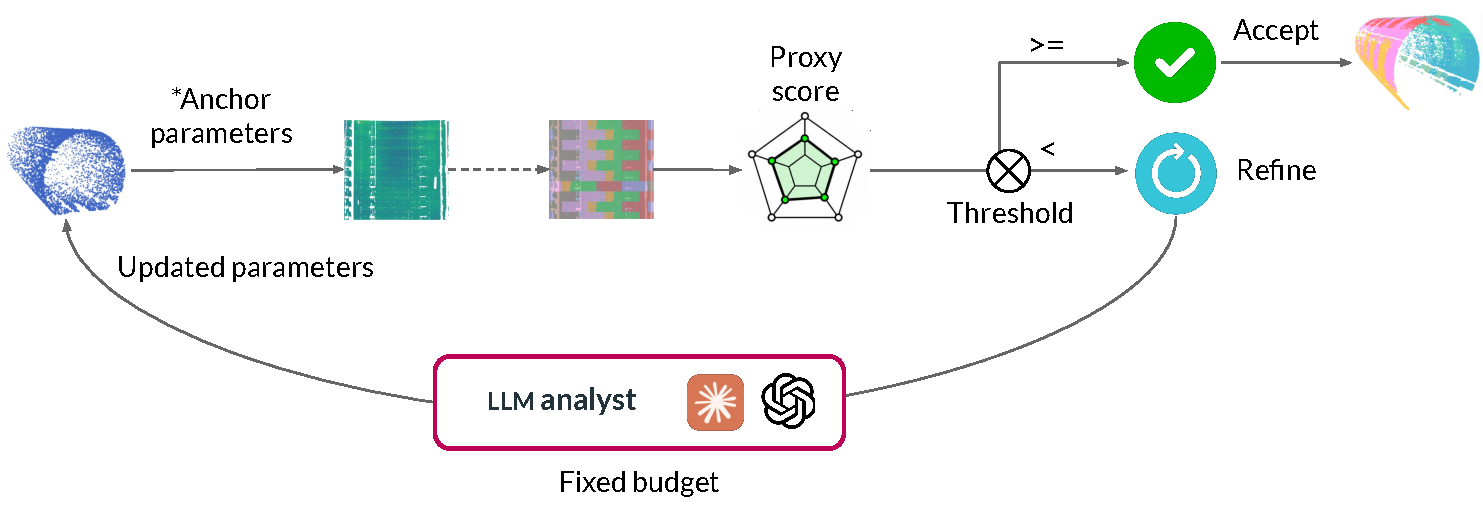
\includegraphics[width=0.9\textwidth]{figures/verification-1.pdf}
\caption{Proof-of-concept proxy verification. Each held-out subset is first
processed with the anchor parameters of its tunnel family and scored by the
learned proxy. Runs scoring at or above the acceptance threshold
($\tau = 0.7$) are accepted directly; otherwise an LLM agent, prompted with
the tunnel ontology, inspects the result and proposes updated parameters. The
loop repeats within a fixed refinement budget, after which the
highest-scoring configuration is retained. Accepted results are subsequently
evaluated against ground truth (mIoU).}
\label{fig:poc-workflow}
\end{figure*}

The final experiment tests whether the frozen proxy can drive a label-free
refinement loop (Fig.~\ref{fig:poc-workflow}). Each of five subsets is first
processed with its family anchor parameters and scored by the proxy. Runs
scoring at or above the acceptance threshold ($\tau = 0.7$) would be accepted
directly; below it, an LLM agent inspects the GT-free intrinsics and
artifacts, diagnoses deviations via the tunnel ontology, and proposes a
bounded multi-stage parameter overlay. Each round is re-scored by the proxy,
and after at most three rounds the highest-proxy configuration is retained.
The acceptance threshold is a deliberately conservative operating point on
the proxy score, distinct from the low-quality alarm threshold
($\tau = 0.495$) validated in Section~\ref{sec:main-results}: the former asks
``is this run good enough to ship without refinement?'', the latter ``is this
run bad enough to flag?''. Ground-truth mIoU is revealed only at final
evaluation and never enters the loop. Given the small sample ($n = 5$), we
report results per case and draw no statistical conclusions beyond
demonstrated feasibility.

\begin{table}[ht]
\caption{Proof-of-concept self-refinement: best-of-three reflection rounds
selected by proxy score, evaluated against ground truth only
afterwards.}\label{tab:poc-results}
\begin{tabular*}{\tblwidth}{@{} l c c c c @{}}
\toprule
Subset & Anchor mIoU & Selected mIoU & $\Delta$mIoU & Improved \\
\midrule
4-4 & 0.347 & 0.700 & $+$0.353 & yes \\
1-5 & 0.549 & 0.782 & $+$0.233 & yes \\
1-4 & 0.556 & 0.596 & $+$0.040 & yes \\
3-5 & 0.588 & 0.628 & $+$0.040 & yes \\
4-3 & 0.516 & 0.508 & $-$0.008 & no \\
\bottomrule
\end{tabular*}
\end{table}

\textbf{Selection by proxy improves four of five subsets.}
Table~\ref{tab:poc-results} summarises the campaign. Selecting the round with
the highest proxy score improves ground-truth mIoU on 4/5 subsets, with gains
from $+$0.040 to $+$0.353; the largest gain (subset 4-4, 0.347
$\rightarrow$ 0.700) doubles segmentation quality on a complex tunnel whose
anchor configuration under-detected ring boundaries. In each improved case
the round selected by proxy also improved ground-truth mIoU.

\begin{figure*}[t]
\centering
\begin{subfigure}{0.32\textwidth}
\centering
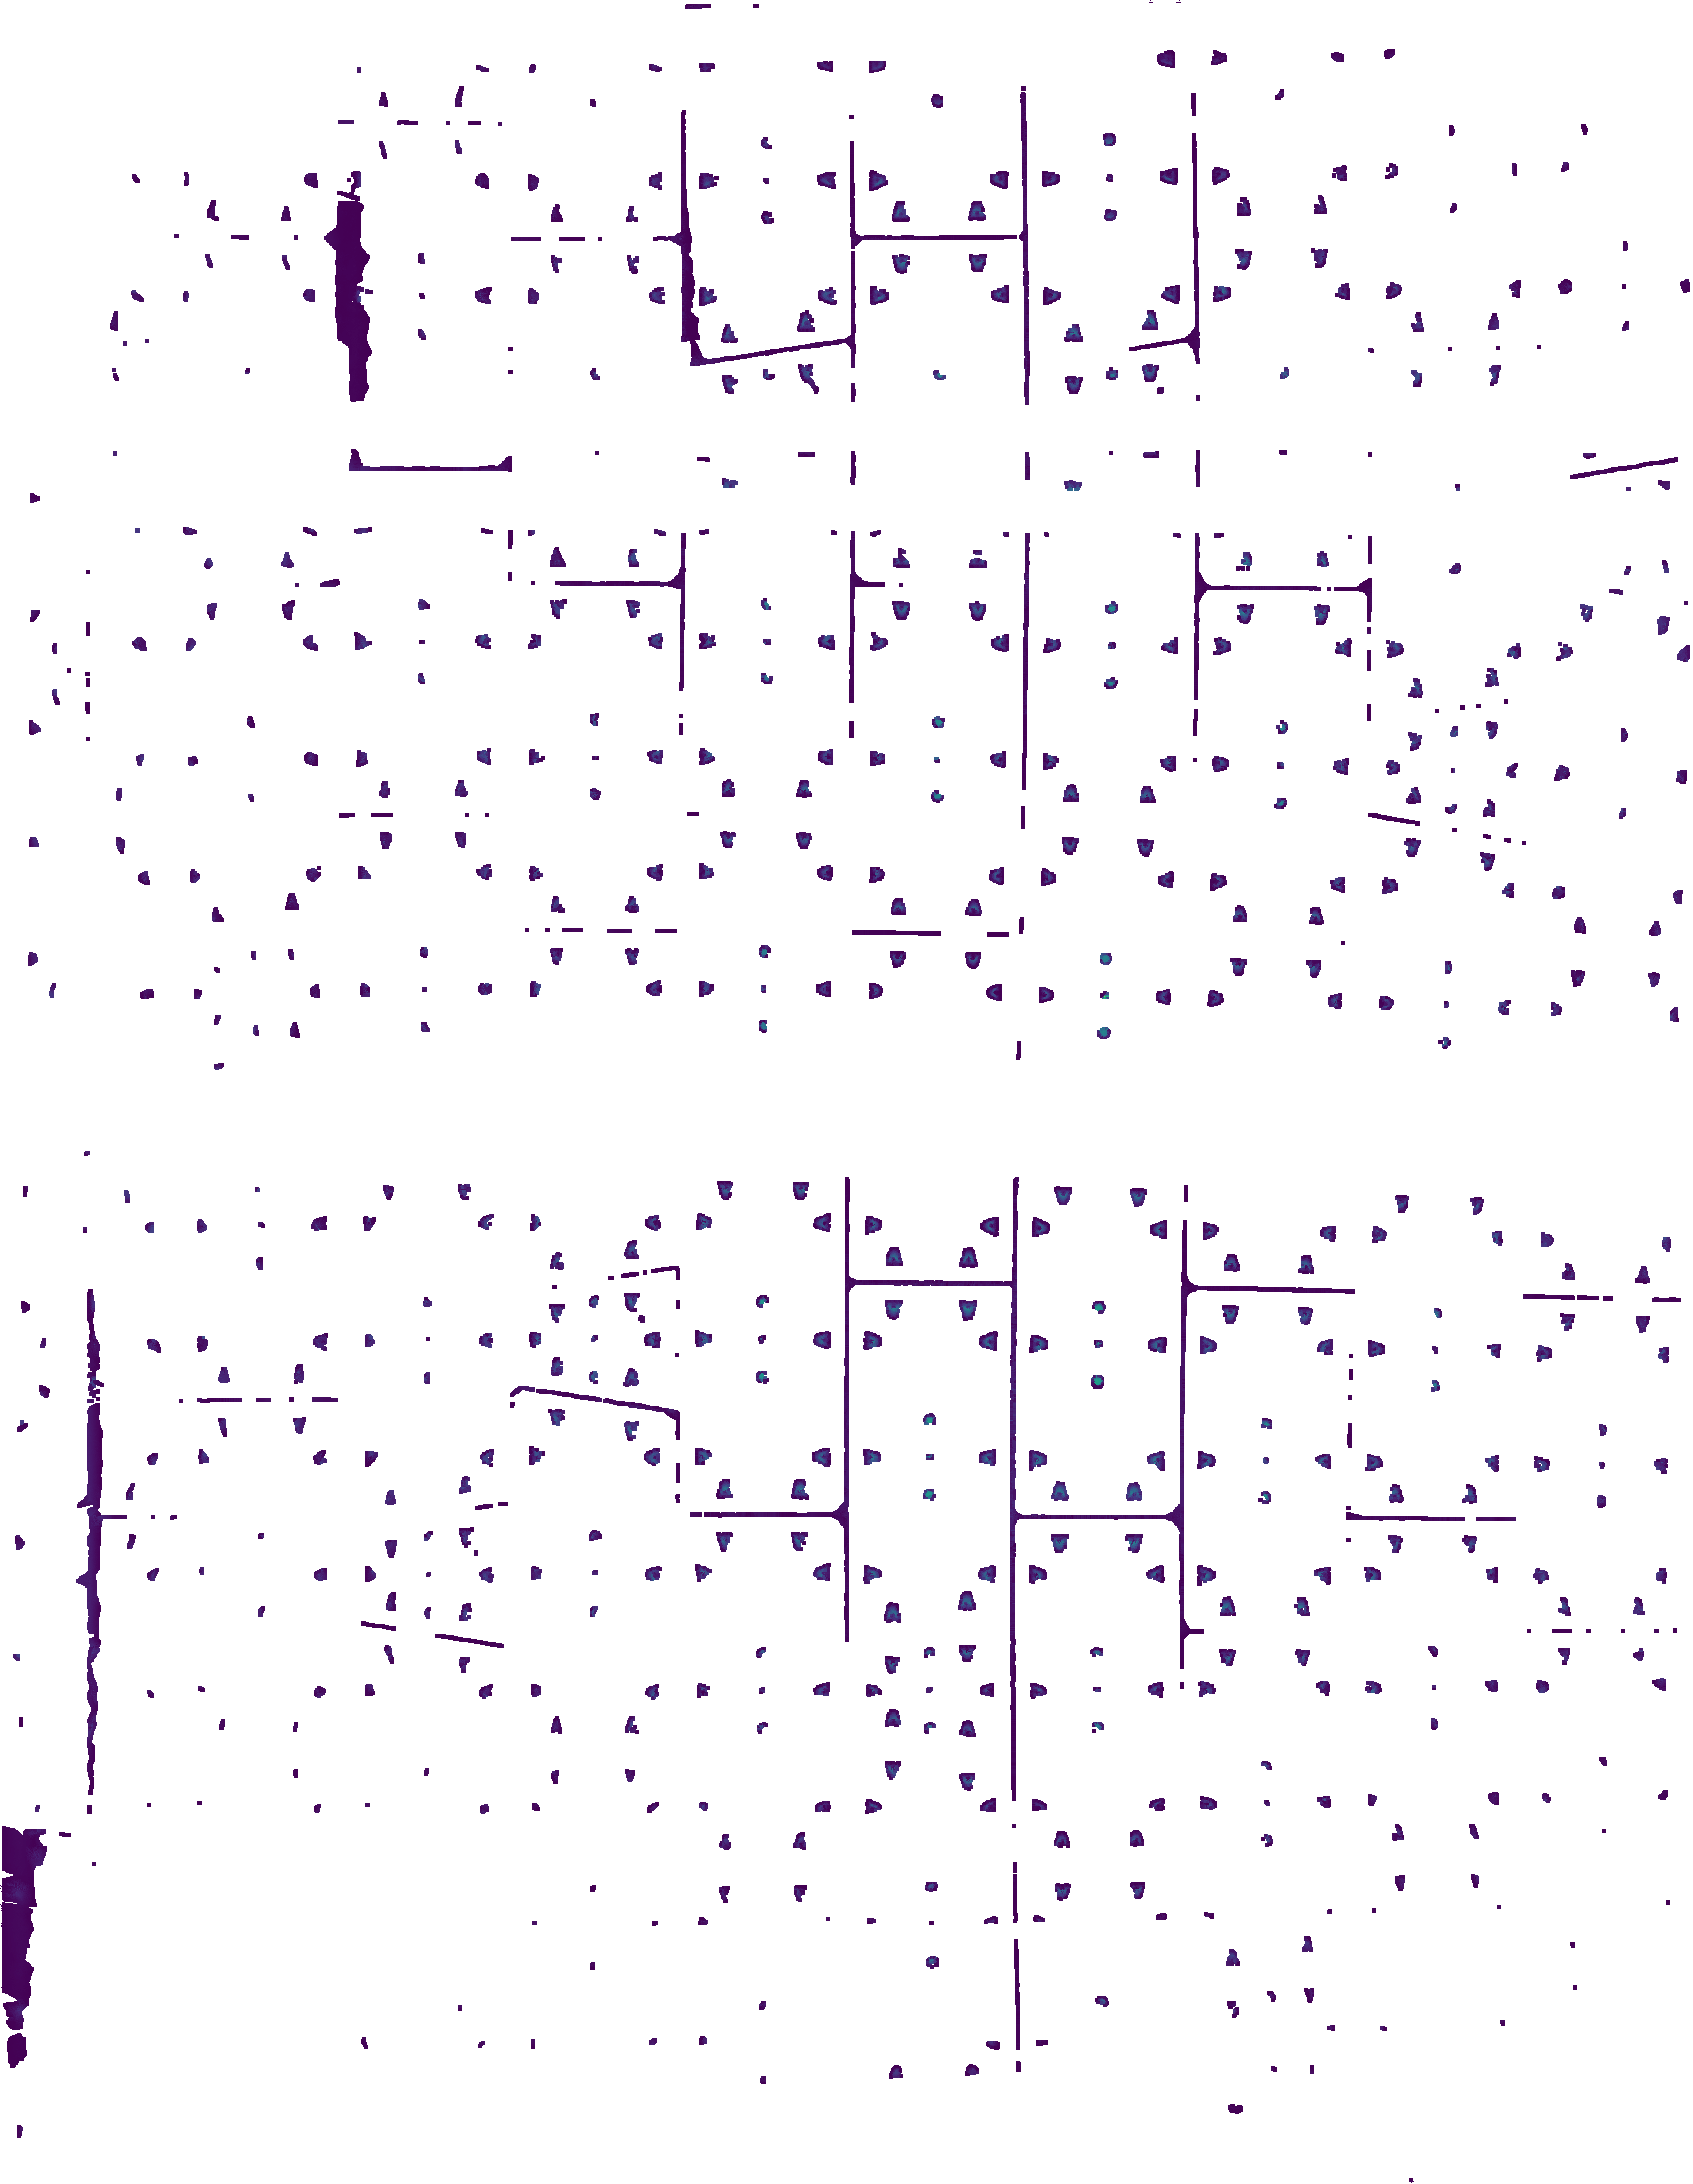
\includegraphics[width=\textwidth]{figures/5-1/low_depth_map.png}
\par\smallskip
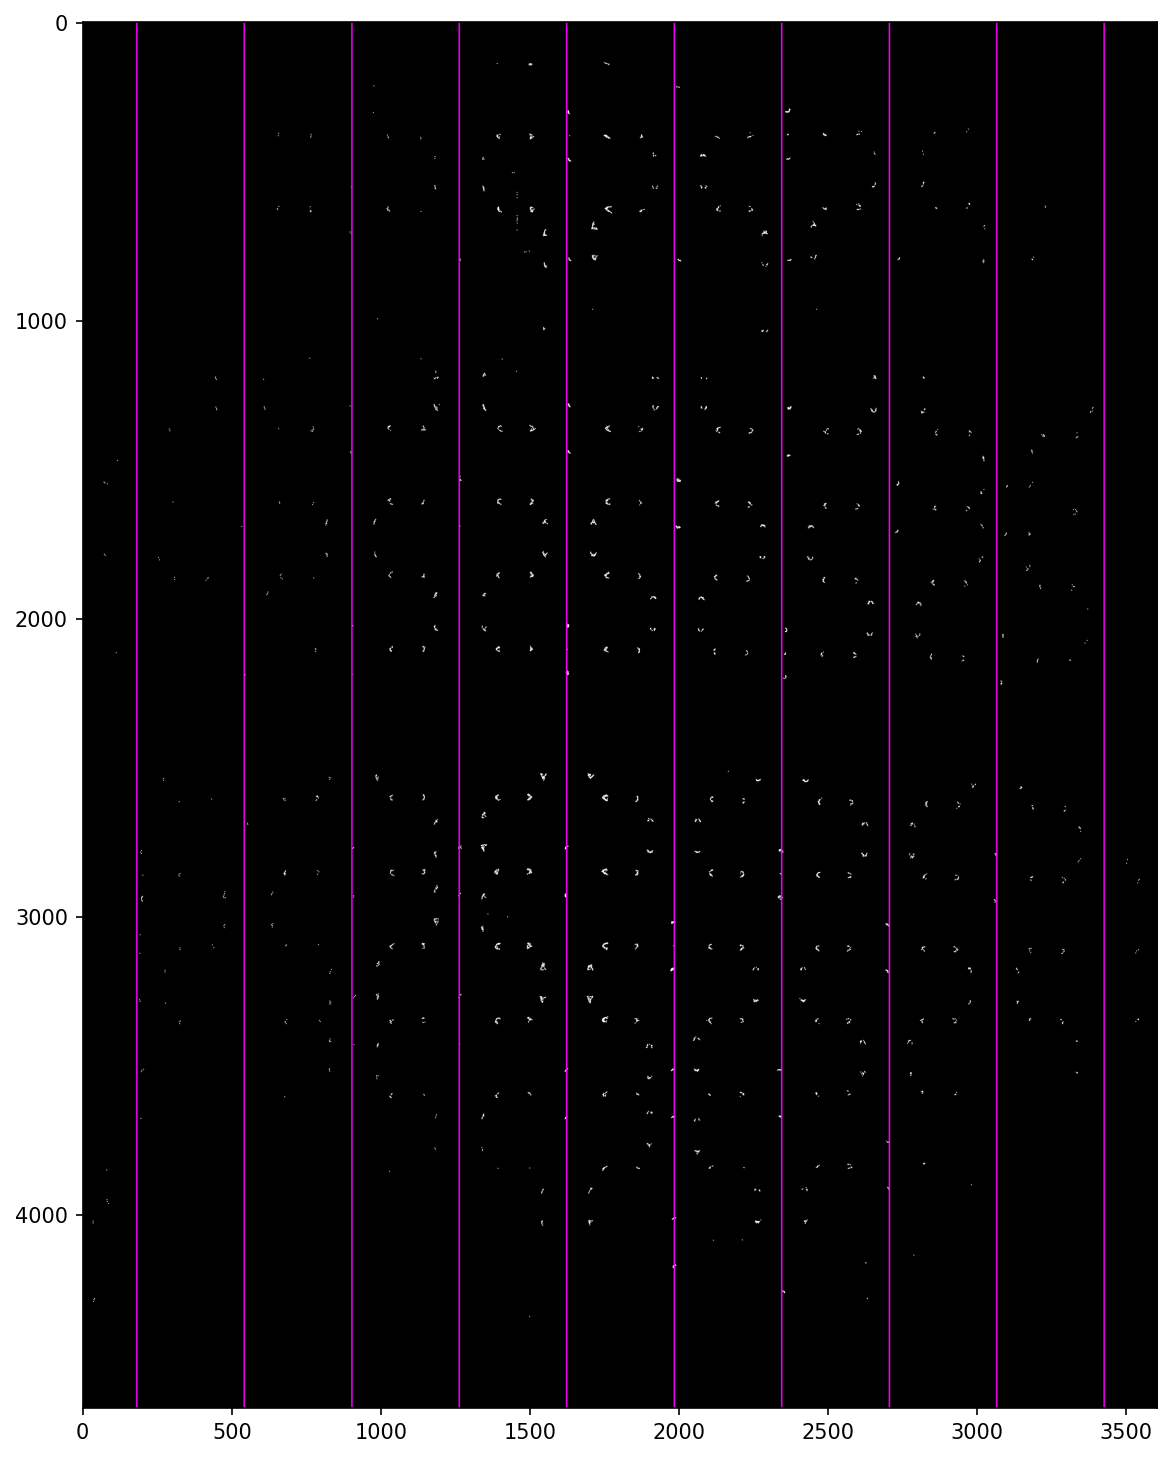
\includegraphics[width=\textwidth]{figures/5-1/low_detected_lines.png}
\par\smallskip (a) Low quality
\end{subfigure}
\hfill
\begin{subfigure}{0.32\textwidth}
\centering
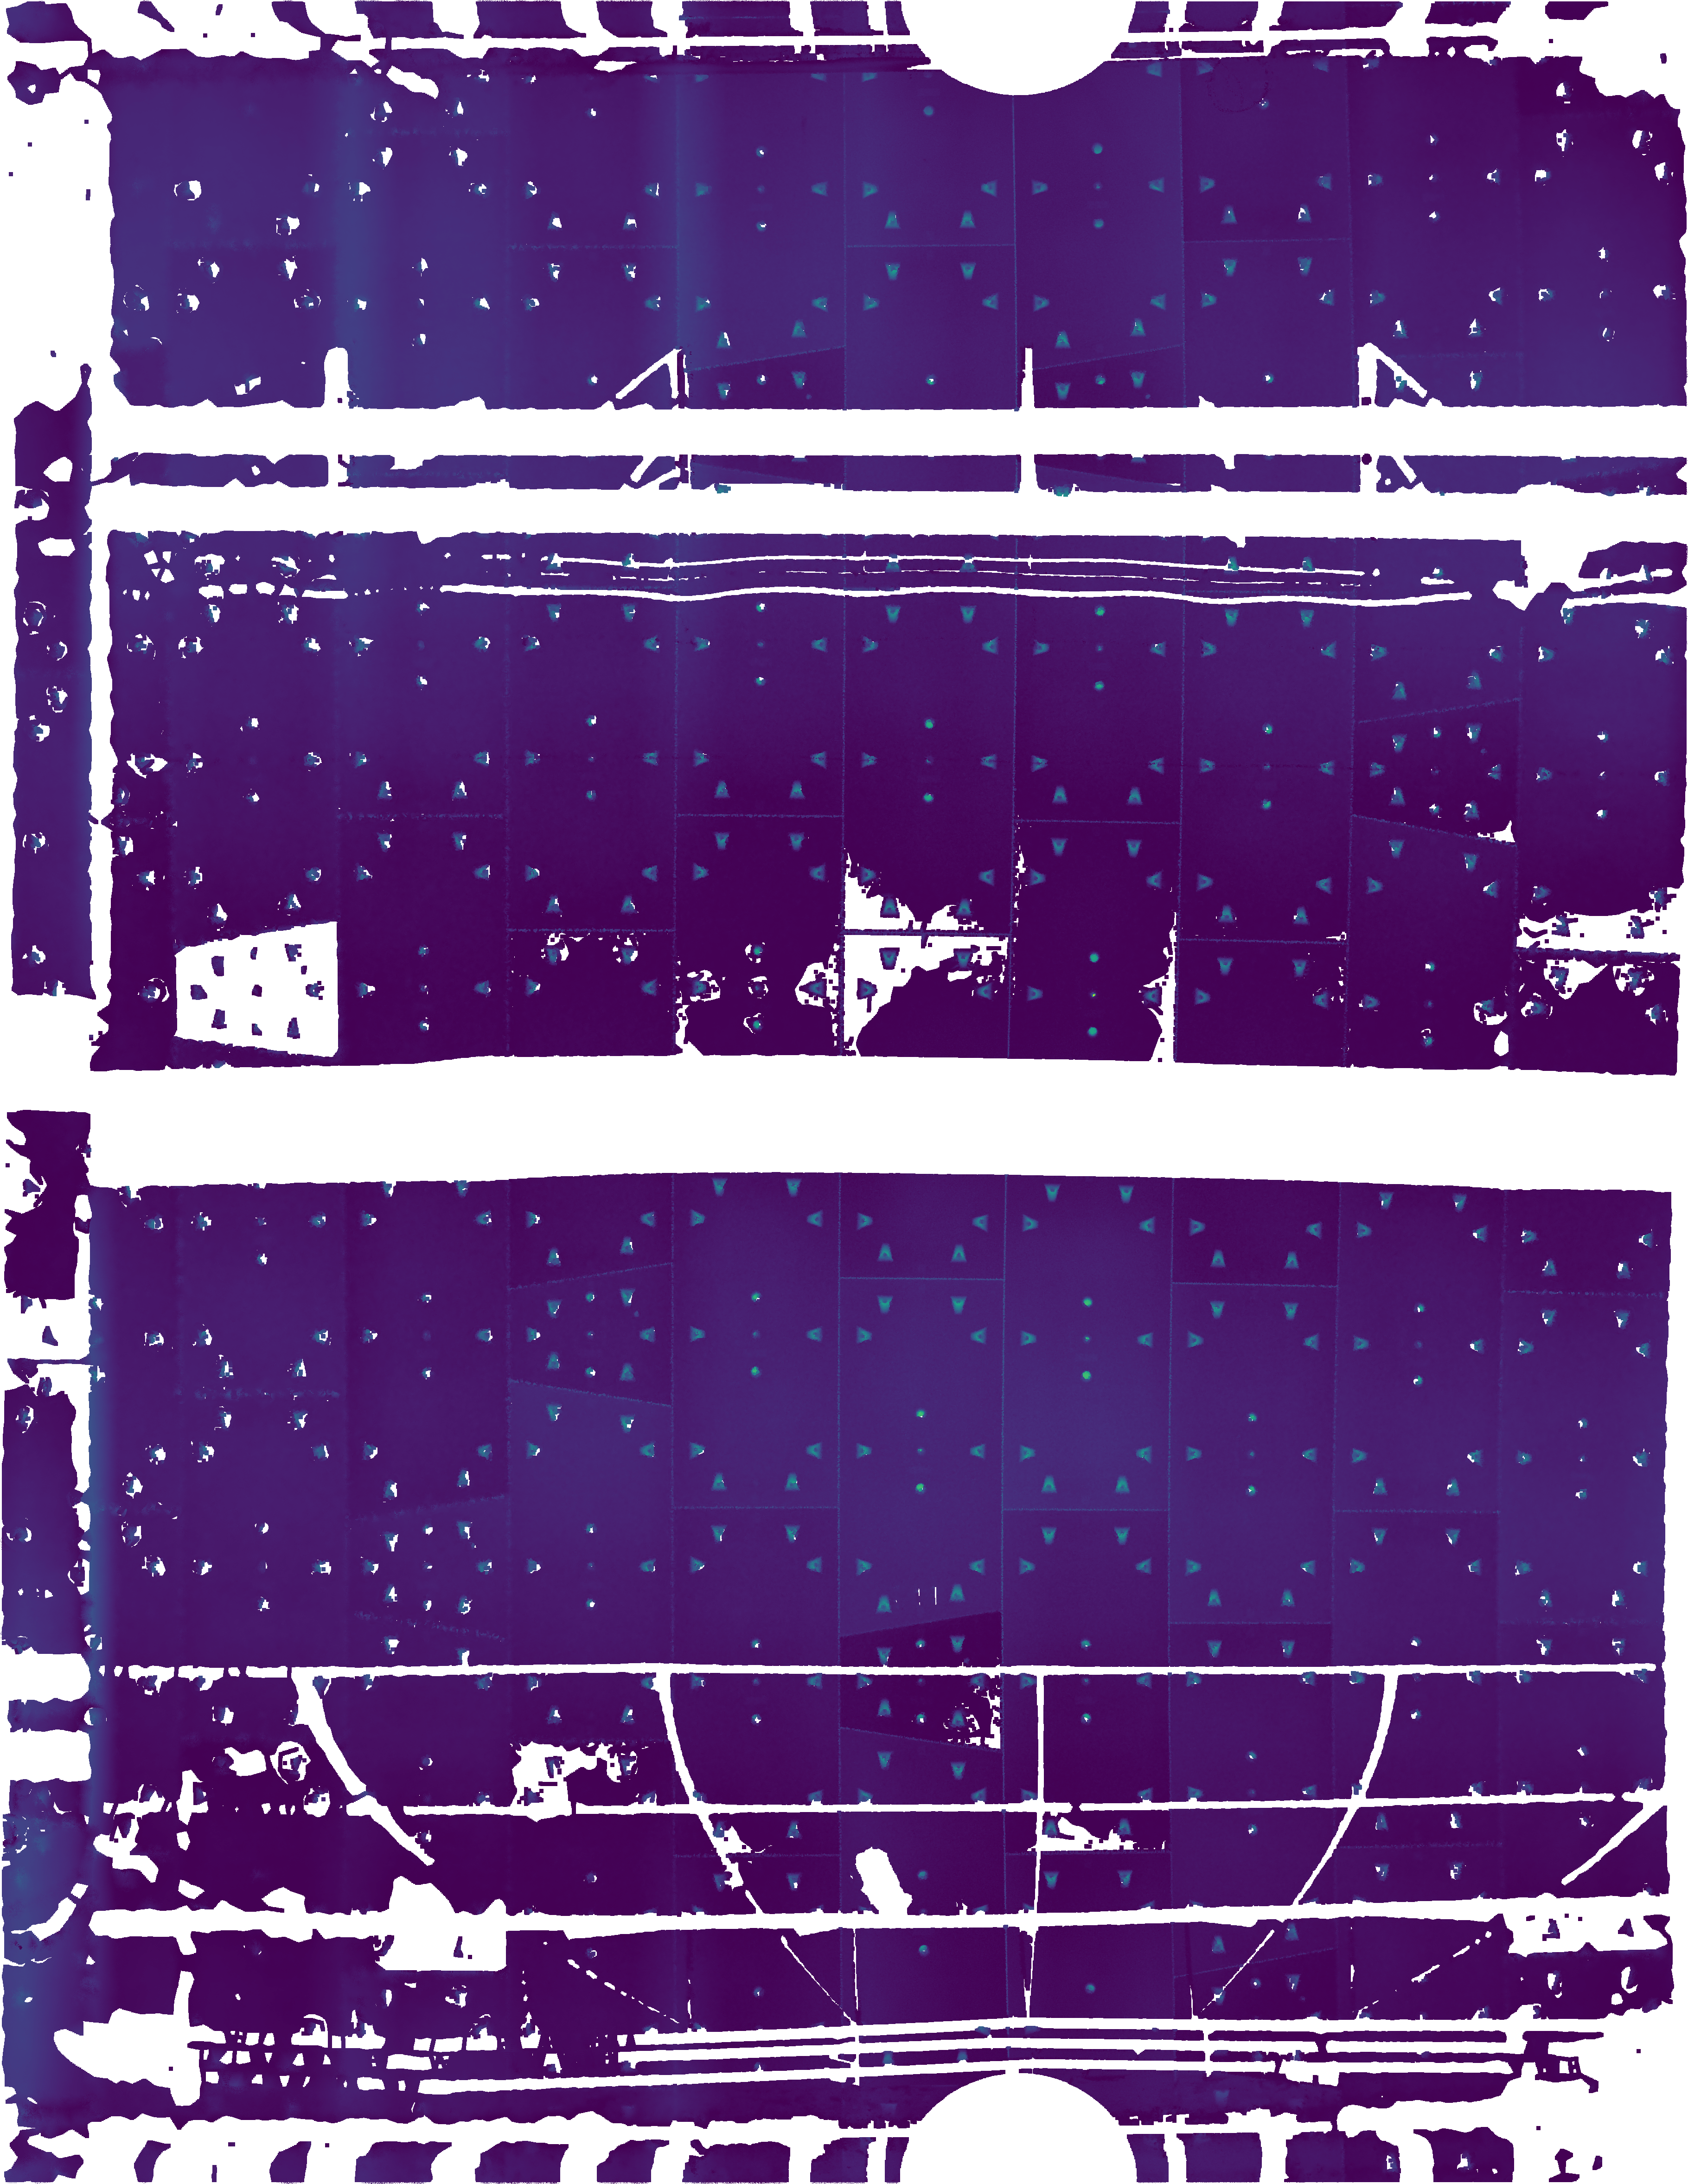
\includegraphics[width=\textwidth]{figures/5-1/mid_depth_map.png}
\par\smallskip
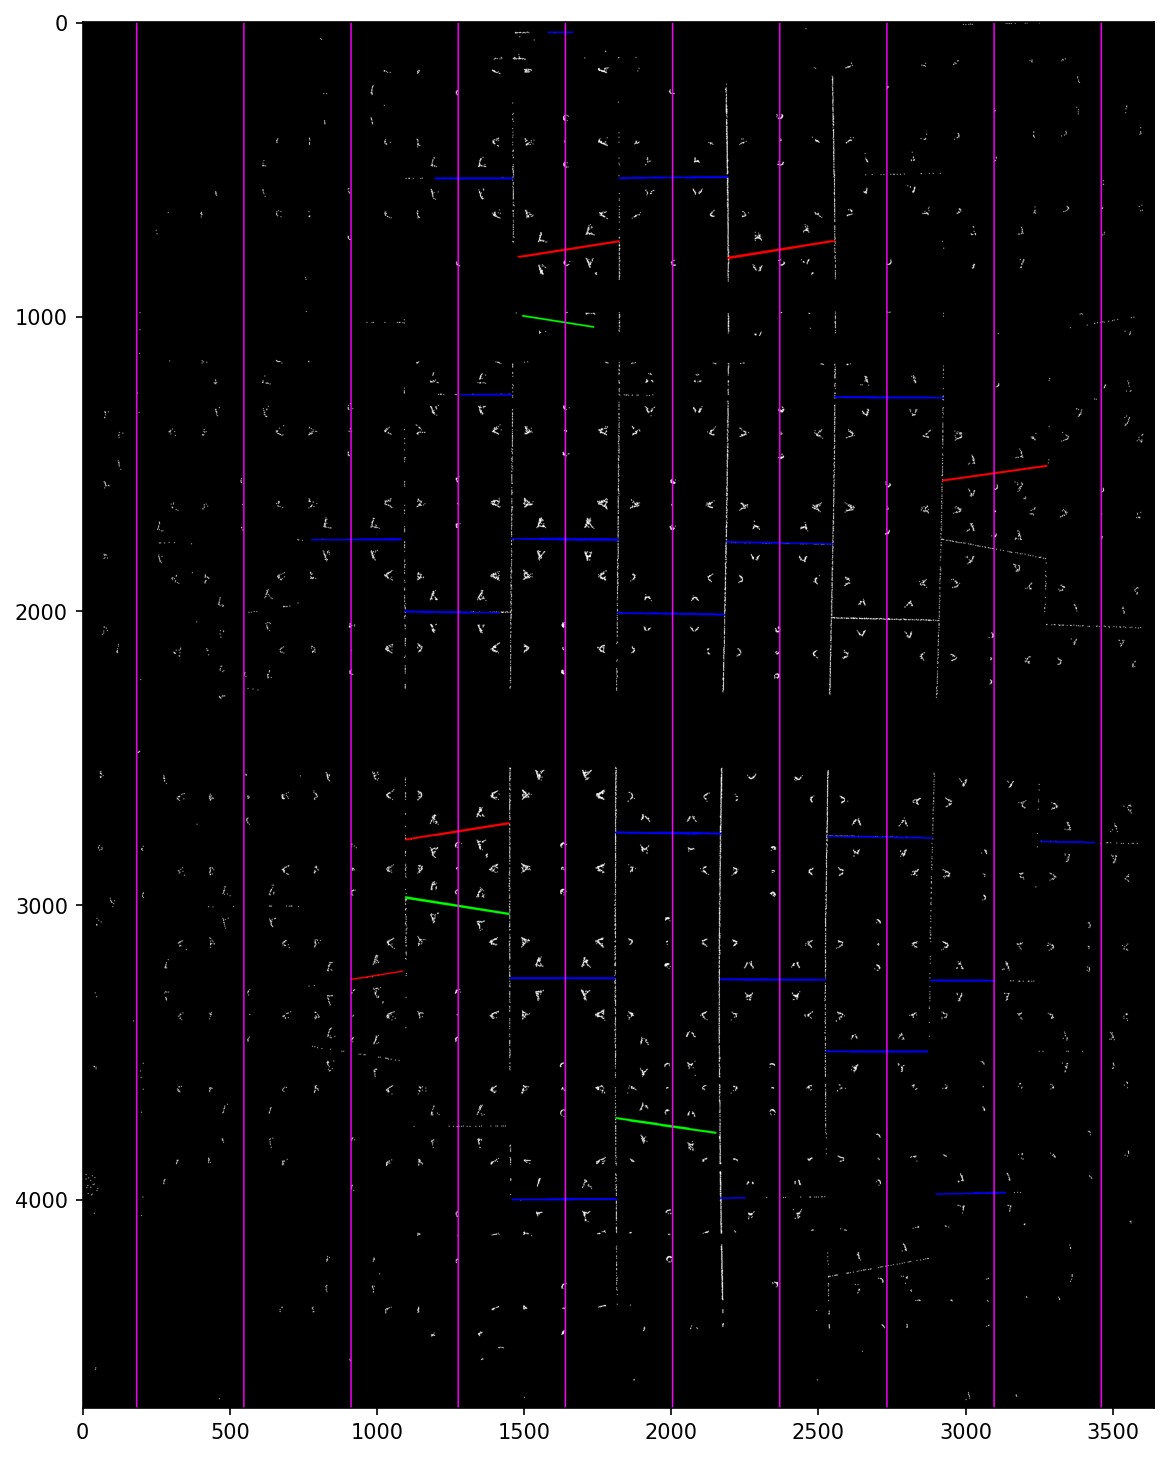
\includegraphics[width=\textwidth]{figures/5-1/mid_detected_lines.png}
\par\smallskip (b) Medium quality
\end{subfigure}
\hfill
\begin{subfigure}{0.32\textwidth}
\centering
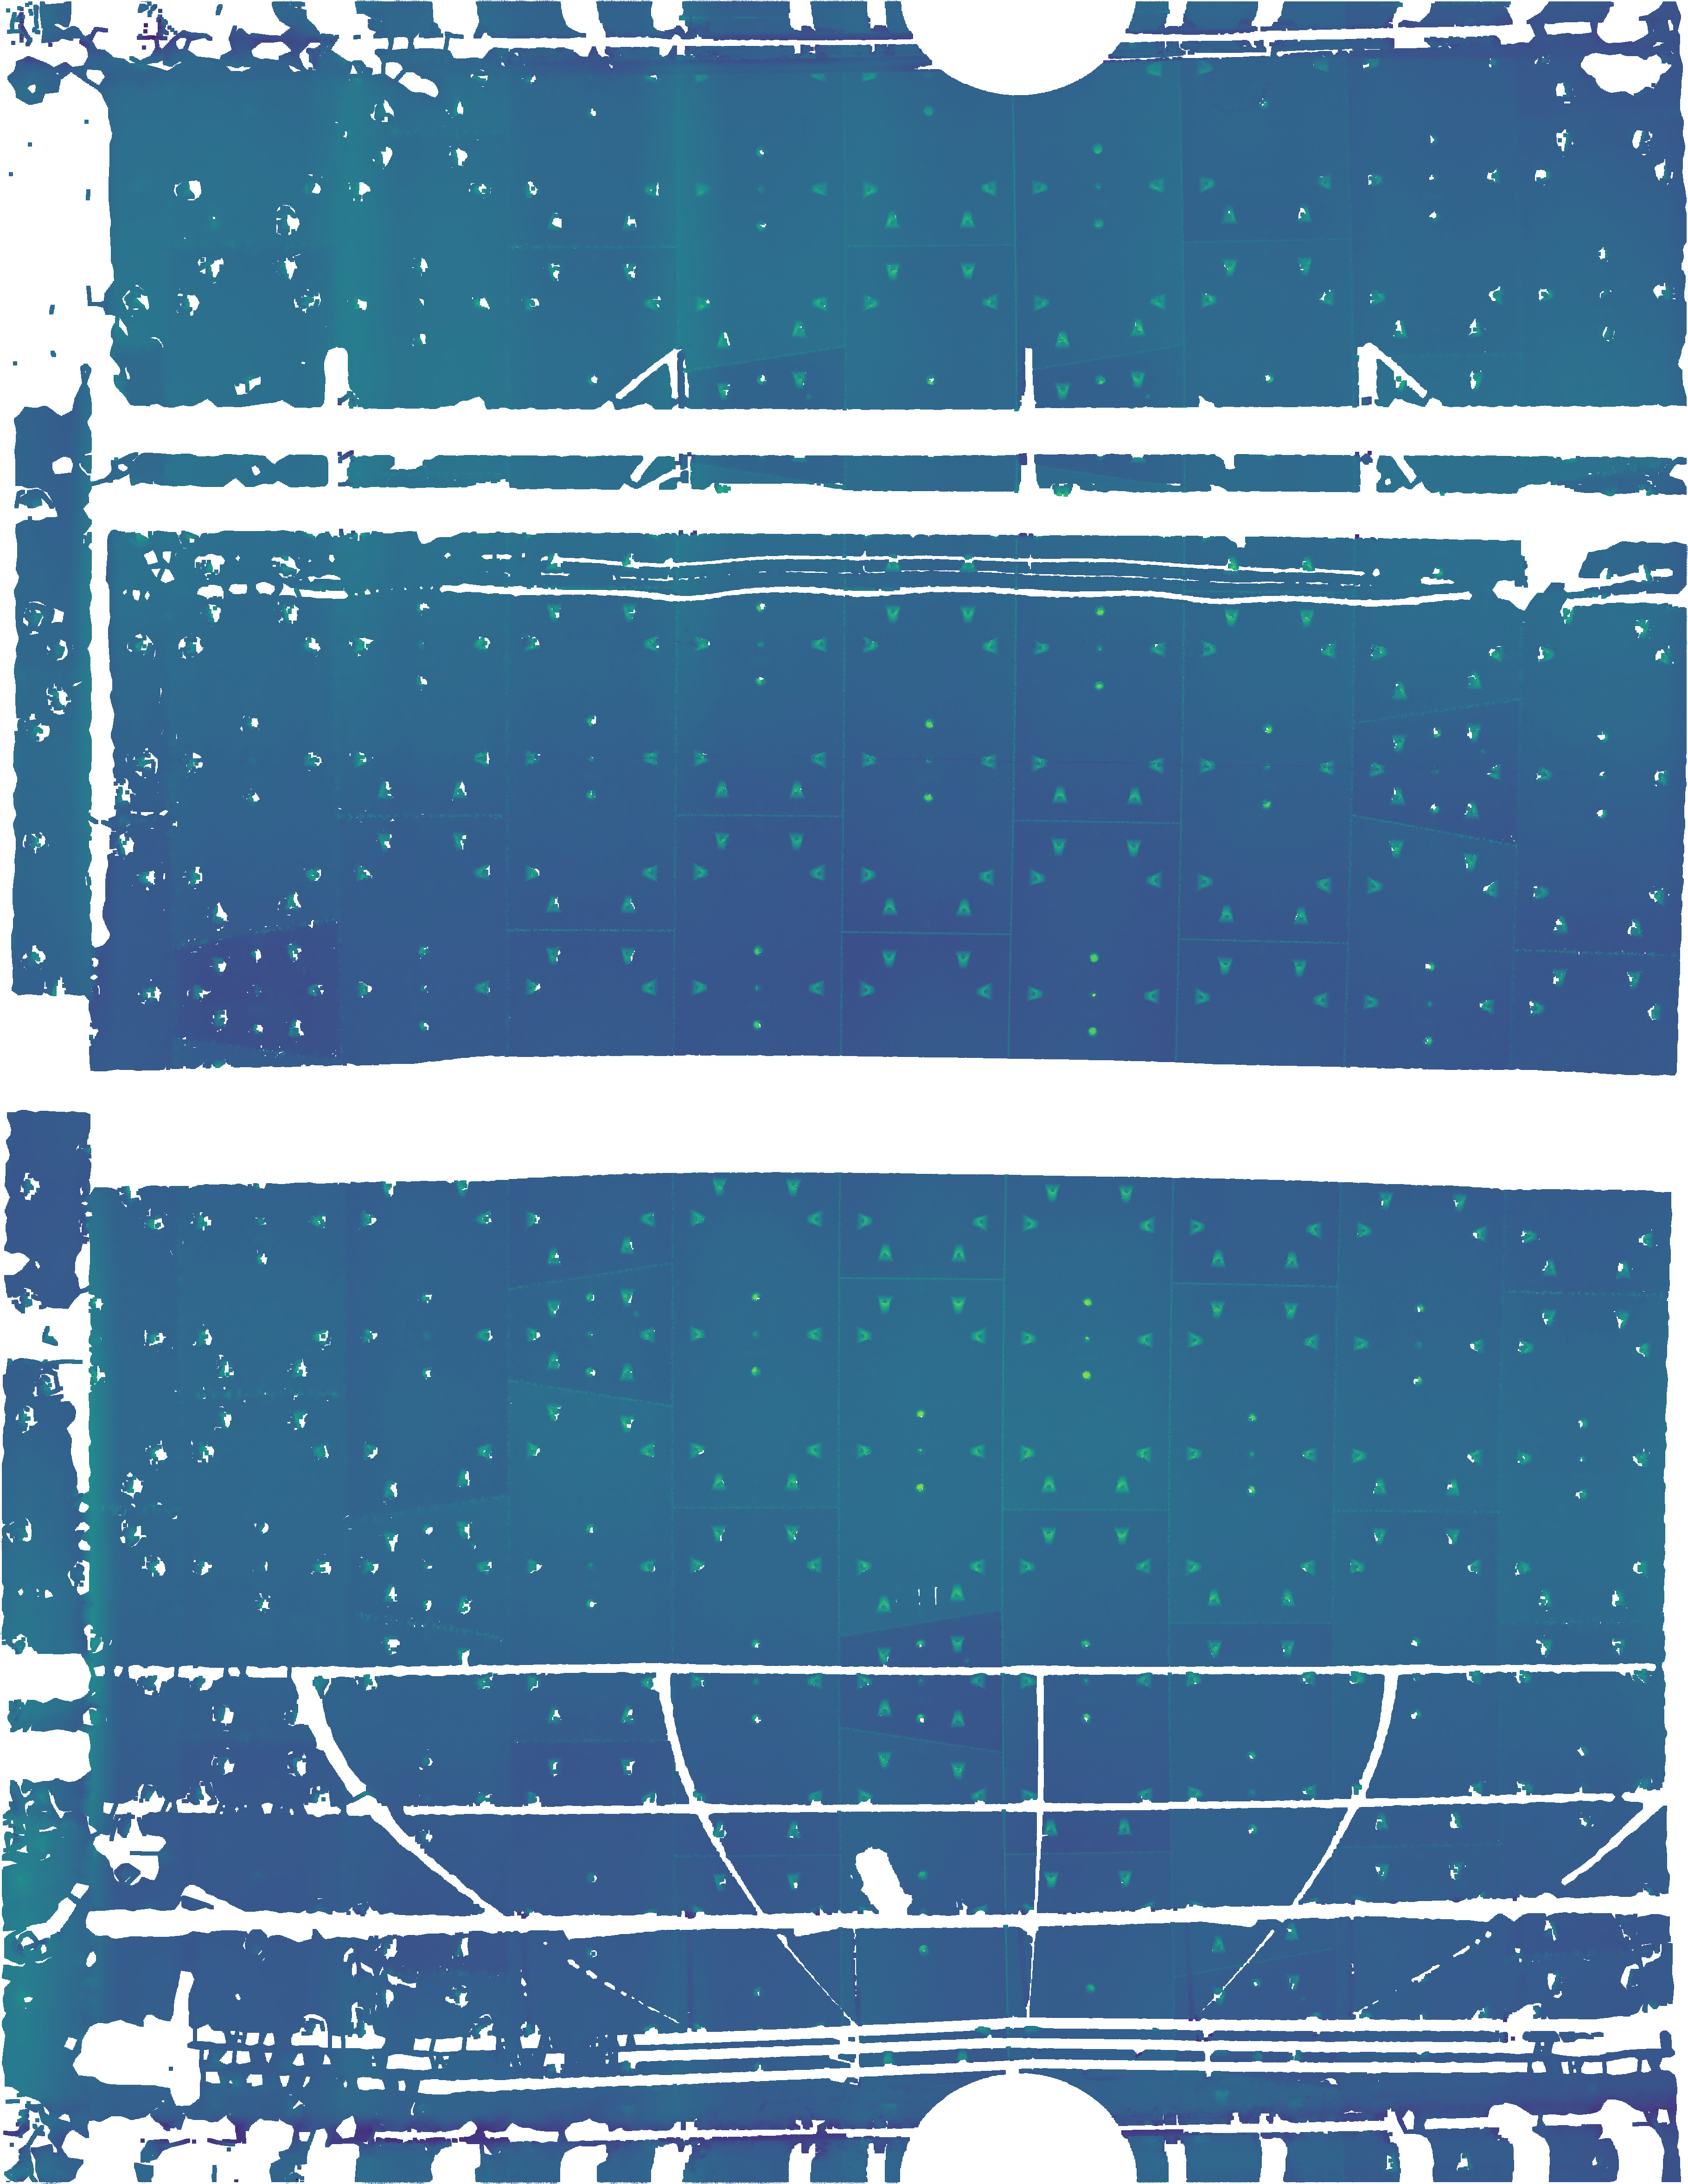
\includegraphics[width=\textwidth]{figures/5-1/best_depth_map.png}
\par\smallskip
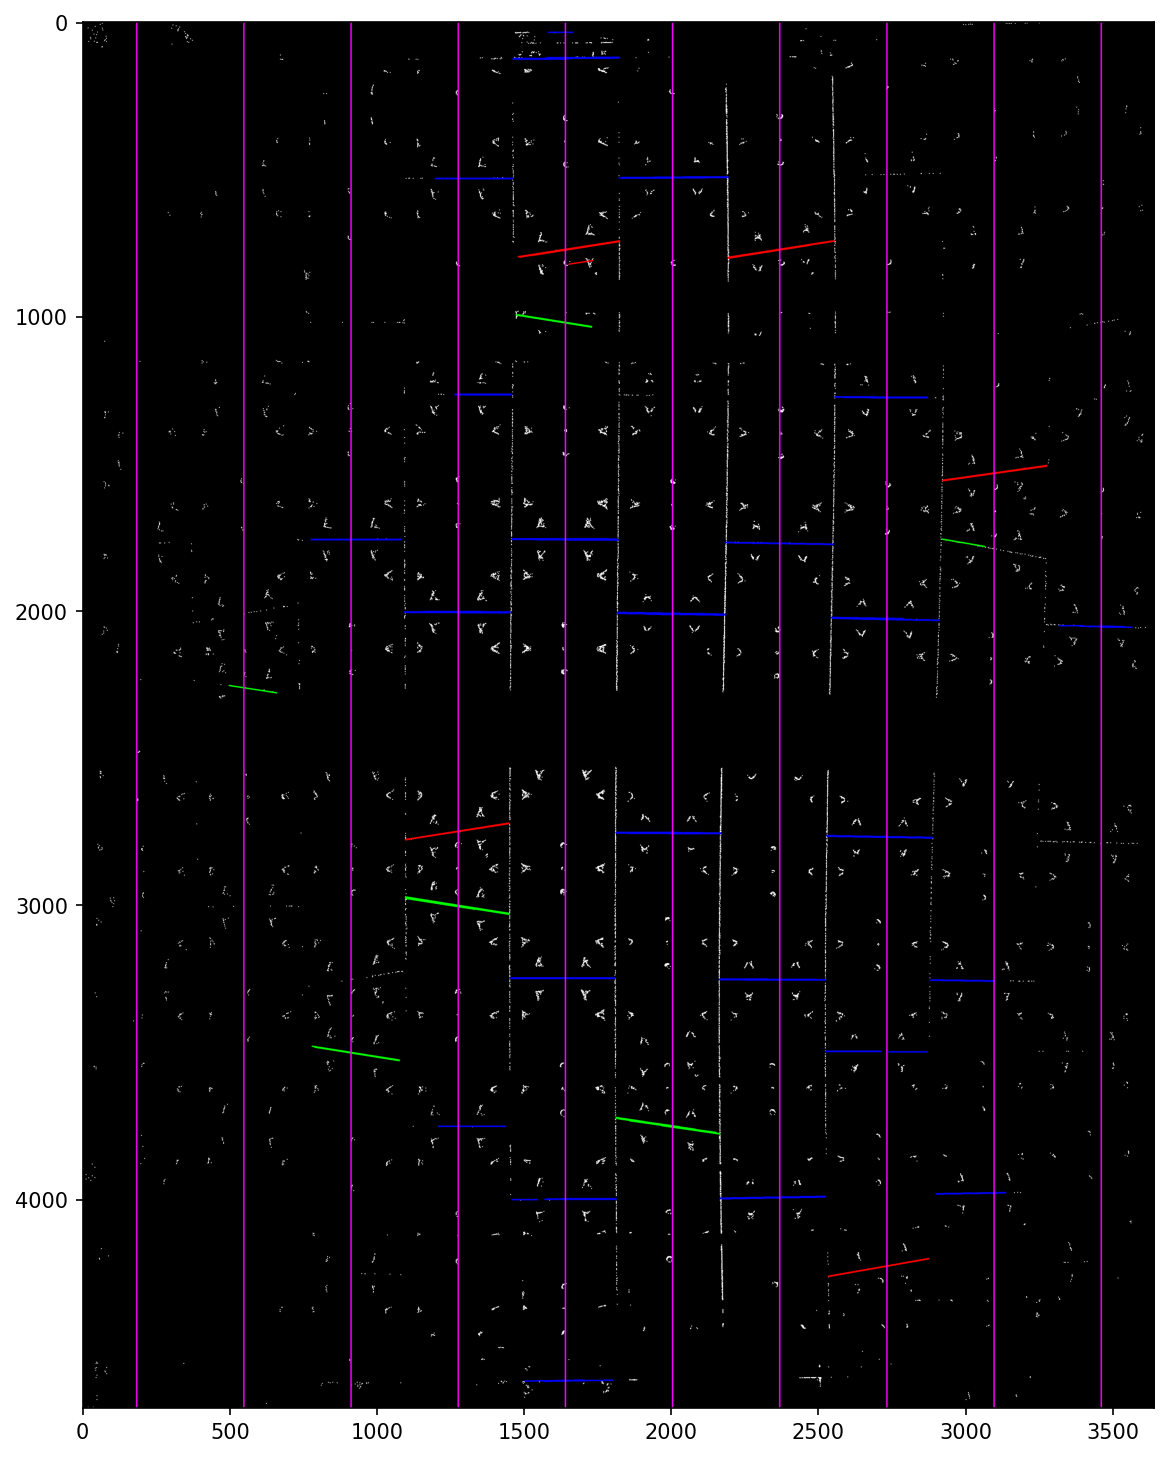
\includegraphics[width=\textwidth]{figures/5-1/best_detected_lines.png}
\par\smallskip (c) High quality
\end{subfigure}
\caption{What the proxy sees: unfolded depth maps (top) and detected joint
lines (bottom) for low-, medium-, and high-quality configurations of a
complex-family subset (5-1). Degraded configurations leave visible traces in
the artifacts --- incomplete depth coverage and irregular or missing joint
lines --- which the evidence and coherence features quantify without labels.}
\label{fig:poc-artifacts}
\end{figure*}

\textbf{Failure analysis: subset 4-3.} The one failure is diagnostic rather
than incidental. A ceiling probe over the stages 2--6 search space shows that
\emph{no} parameter overlay available to the reflection loop beats the anchor
on 4-3 (best manual configuration: $-$0.001; reflection best: $-$0.008): the
binding defect is the stage-1 centreline, whose recentring residual of
23.2\,cm distorts the unfolded geometry before any downstream parameter acts.
This quantity is invisible to the lean proxy --- substituting a healthy
residual into the 4-3 feature vector changes the prediction by exactly zero,
since the stage-1 candidates were pruned during feature ablation
(Section~\ref{sec:proxy-ablation-results}). When the loop is re-run with
stage~1 unlocked, changing the unfolding seed alone reduces the residual to
5.2\,cm and raises mIoU to 0.554 ($+$0.038 over the anchor), and all three
stage-1-aware rounds beat the anchor. The proxy thus delimits its own scope:
it reliably scores what the depth-map and segmentation artifacts reveal
(Fig.~\ref{fig:poc-artifacts}), and the 4-3 case identifies stage-1 geometry
auditing as the concrete extension required for a fully reflective agent.

\textbf{Scope of the claim.} This PoC is intended to demonstrate the proxy's
potential as a self-refinement signal for reflective LLM agents or
reinforcement learning, not to establish a general adaptation method: the
subsets were chosen to span families and failure modes, the refinement budget
was fixed at three rounds, and no hyperparameters were tuned on the outcome.
Within that scope, the loop shows that a frozen, five-feature linear proxy is
informative enough to select better configurations without any deployment
labels --- and, through its one failure, shows precisely where richer stage-1
evidence is needed.


\section{Discussion}\label{sec:discussion}

The results support a mechanism-level claim: a frozen, five-feature linear model over stage-observable metrics can serve as a GT-free control signal for a multi-stage tunnel segmentation pipeline. Labels enter only once, at design-time calibration on Bayesian-exploration trials; every deployment-time decision---score, rank, accept, flag, or select between refinement rounds---is made from intermediate artifacts alone, and every decision is auditable because the model is linear with inspectable coefficients.

\subsection{Key findings}

Two findings organise the results. First, the quality signal lives in the \emph{form} of the result more than in the quality of the artifacts: coherence features (led by segment-mask fill rate) dominate both the ablation and the frozen coefficients, and the combined ten-feature set generalises \emph{worse} across families than coherence alone until leave-one-out pruning removes the anchor-specific features (LOLO Spearman 0.537 $\rightarrow$ 0.717). Pruning is therefore not a parsimony preference but the mechanism that converts in-sample fit into cross-family transfer. Second, one pooled model is the right deployment choice: per-family refits of the same lean features edge the pooled model on absolute fidelity (MAE 0.057 vs.\ 0.071) but lose alarm recall (0.96 vs.\ 1.00), and a single calibration is operationally simpler across the three lining families.

For practice, the workflow implication mirrors the design: an engineer calibrates once per pipeline release---anchor selection, bounded exploration, ablation, freeze---and thereafter receives a per-run quality estimate and alarm at negligible cost. The PoC shows the same signal can drive refinement: selecting LLM-proposed overlays by proxy score improved four of five subsets without any label access. The single failure (4-3) is itself informative: the loop's ceiling probe and the proxy's provable insensitivity to the pruned stage-1 residual localise the defect to centreline geometry, turning a miss into a concrete specification for the next capability rather than an unexplained error.

\subsection{Positioning relative to prior deployment control}

Comparisons here are about operating points, not accuracy leaderboards. Relative to static SAM4Tun, Proxy4Tun adds an explicit accept/refine/flag channel without deployment labels. Relative to one-shot LLM adapters such as R4Tun, it adds a calibrated numeric critic, so refinement can be verified rather than merely proposed. Relative to generic segmentation QC~\cite{valindria2017rca,fournel2021segmentationQC} and uncertainty estimation~\cite{gal2016dropout,lakshminarayanan2017deepEnsembles}, the feature set is specialised to cylindrical unfolding and segmental lining grammars, and the calibration cost is three labelled anchor tunnels rather than a labelled validation stream. BO remains offline experience generation~\cite{snoek2012practicalBO,garnett2023bayesianOptimization}; no labels or surrogates are queried at runtime.

\subsection{Limitations}

The frozen proxy has a demonstrated blind spot: stage-1 geometry. The two stage-1 audit features carried too little standalone signal to survive pruning, so centreline defects (as on subset 4-3) are invisible to the score; stage-1 gating or richer geometric evidence is required before the loop can be considered fully reflective. Calibration rests on one expert-tuned anchor per family, and transfer is demonstrated within Seg2Tunnel's three families under the SAM4Tun stage graph; different sensors, lining grammars, or pipelines require re-calibration, though the protocol itself (bounded exploration, ablation, permutation control, freeze) is pipeline-agnostic. The phase-coherence check is reliable only on regular linings, where a repeating stagger exists. Finally, the self-refinement PoC covers five subsets with a three-round budget and a single agent configuration; it demonstrates feasibility, not a validated adaptation method.

\section{Conclusions}\label{sec:conclusions}

This paper presented Proxy4Tun, which calibrates a ground-truth-free quality proxy for segmental tunnel-lining segmentation from design-time Bayesian exploration and deploys it, frozen, as an auditable control signal. Space-filling exploration of the bounded parameter space around one expert-tuned anchor per lining family produced 40 labelled trials per family spanning healthy to degraded configurations; feature ablation over evidence and coherence metrics distilled these into a five-feature pooled Ridge proxy with a calibrated alarm.

The main findings are:
\begin{itemize}
\item On 27 held-out subsets (54 scored runs), the frozen proxy tracked GT mIoU with Spearman 0.848 and MAE 0.071, ranked the sibling anchor above a known-bad configuration on every subset, and flagged all 27 known-bad runs with zero false alarms.
\item Coherence features carry most of the quality signal, and leave-one-out pruning---not feature accumulation---delivers cross-family transfer; the deployed five-feature model outperforms the full ten-feature candidate set out of family.
\item A single pooled model matches per-family refits where it matters: per-family calibration gains 0.014 MAE but loses alarm recall, so one unified proxy serves all three lining families.
\item As a proof of concept, selecting LLM-proposed bounded parameter overlays by proxy score improved mIoU on four of five subsets ($+$0.040 to $+$0.353) without any deployment labels; the single failure was traced to a stage-1 centreline defect outside the proxy's feature scope.
\end{itemize}

The approach is limited by its stage-1 blind spot, its single-anchor-per-family calibration, and the scope of the PoC; absolute segmentation quality remains bounded by the underlying SAM4Tun stages. Future work will add stage-1 geometry auditing (residual and orientation gates) to close the demonstrated blind spot, extend the reflective agent to full campaigns across the holdout panel, use the frozen proxy as a reward signal for reinforcement-learning-based tuning, and evaluate multi-anchor calibration for families with larger within-family variation. These results indicate that intrinsic, stage-observable metrics---calibrated once and frozen---can serve as an auditable control plane for foundation-model tunnel pipelines when ground truth is unavailable.

\section*{Data availability}

The source code, parameter snapshots, BO experience tables, and evaluation scripts will be released upon publication. The Seg2Tunnel dataset is publicly available~\cite{lin2024seg2tunnel}.

\section*{Declaration of competing interest}

The authors declare that they have no known competing financial interests or personal relationships that could have appeared to influence the work reported in this paper.

\bibliographystyle{model1-num-names}
\bibliography{references}
\end{document}
